 \chapterimage{chapter_head_1.pdf} % Chapter heading image
\chapter*{Propositional and First-order Logic Primer}
\addtocounter{chapter}{1} % Manually increment the chapter counter
\markboth{\sffamily\normalsize\bfseries Propositional and First-order Logic Primer}{} % Set the chapter header
\addcontentsline{toc}{chapter}{\textcolor{ocre}{Propositional and First-order Logic Primer}}

%%%% BEGIN %%%
\section*{A Primer on Introduction and Elimination Rules in (Classical) First Order Logic}

This appendix will briefly introduce the rules for natural deduction in propositional logic and then add rules for universal and existential quantifiers to arrive at the rules for classical first-order logic. The presentation closely follows one given by \href{https://markjago.net/}{Dr. Mark Jago} on his \href{https://www.youtube.com/@AtticPhilosophy}{\textit{Attic Philosophy}} YouTube channel (some sections are more or less a transcription of his explanations!). I encourage you to engage with his channel as it is a wonderful (and free) learning resource for all sorts of topics in logic and philosophy. 

The introduction and elimination rules will be presented using Fitch notation, as is quite common in many introductory logic courses in the U.S. and U.K. Towards the end, a brief discussion on Intuitionistic logic, how it relates to classical logic, and where they disagree, will be provided. We will also provide a brief primer on ``Second Order Logic" which is the logic you have used all along in this algebra text.

In these discussions, the turnstile symbol\footnote{For those who are interested, $\vdash$, the turnstile, represents syntactic consequence (or "derivability"). In other words it shows that one string can be derived from another in a single step according to the transformation rules (i.e. the syntax) of some formal theory. This is in contrast to semantic consequence which is denoted with the double turnstile $\vDash$. One says that $S$ is a semantic consequence of $T$, or $T\vDash S$, when all possible valuations in which $T$ is true, $S$ is also true. For propositional logic (i.e. without quantifiers), it can be shown that semantic consequence $\vDash$ and derivability $\vdash$ are equivalent to one-another. That is, propositional logic is sound ($\vdash$ implies $\vDash$) and complete ($\vDash$ implies $\vdash$)} ``$\vdash$", in the context $T \vdash S$ can be taken to mean ``$S$ is provable from $T$" or ``$S$ can be derived from $T$ "\footnote{Others might say $T\vdash S$ means that there is a construction (a proof) that transforms a proof of $T$ into a proof of $S$. In other words, if you have a proof of $T$, then you can construct a proof of $S$ using this transformation.}.

\section{Introduction and Elimination Rules for Propositional Logic}
To begin we will focus on the introduction and elimination rules for the primitive logical connectives (and, or, not, if-then, if-and-only-if). In general each has at least one introduction rule and at least one elimination rule, some have more (e.g. $A\wedge B$ can be eliminated by inferring $A$ or by inferring $B$).

\subsection{Introduction and Elimination rules for Conjunction ($\wedge$) :}
Let's begin by looking at conjunction (i.e. ``and" represented by the wedge symbol ``$\wedge$"). We will provide the rule for introducing a conjunction into a proof and a pair of rules for eliminating a conjunction from a proof.
\subsubsection{Conjunction Introduction Rule ($\wedge I$)}
If we managed to establish $A$ in our proof (either by deductions or as an assumption) and we managed to establish $B$ in our proof, then we can add $A\wedge B$. This is the introduction rule for logical conjunction (a.k.a. the ``and" introduction rule).
\begin{equation}
    \begin{nd}
        \have[m]{1} A
        \have[n]{2} B
        \have[~]{} {A\wedge B} \ai{1,2}
    \end{nd} \nonumber
\end{equation}
\subsubsection{Conjunction Elimination Rules ($\wedge E1$ and $\wedge E2$)}
If we managed to establish $A\wedge B$ in our proof, we can eliminate it in one of two ways. We can eliminate the ``and" and introduce $A$ into our proof
\begin{equation}
    \begin{nd}
        \have[m]{1} {A\wedge B}
        \have[~]{} A \ae{1}
    \end{nd} \nonumber
\end{equation}
or we can eliminate the ``and" and introduce $B$ into our proof
\begin{equation}
    \begin{nd}
        \have[m]{1} {A\wedge B}
        \have[~]{} B \ae{1}
    \end{nd} \nonumber
\end{equation}
These two together are the ``and" elimination rules ($\wedge E$)

\subsection{Introduction and Elimination Rules for Disjunction ($\lor$)}
Next we will look at the disjunction connective (i.e. ``or" represented by the upside-down wedge symbol ``$\lor$")
\subsubsection{Disjunction Introduction Rules ($\lor I1$ and $\lor I2$)}
If we have $A$ in a proof, we can introduce disjunction:
\begin{equation}
    \begin{nd}
        \have[m]{1} {A}
        \have[~]{} {A\lor B} \oi{1}
    \end{nd} \nonumber
\end{equation}
i.e. from $A$ we can deduce $A$ or $B$ ... and we can also do it the other way around:
\begin{equation}
    \begin{nd}
        \have[m]{1} {A}
        \have[~]{} {B \lor A} \oi{1}
    \end{nd} \nonumber
\end{equation}
From $A$ we can deduce $B$ or $A$. Together these two are the ``or" introduction rules $\lor I$
\subsubsection{Disjunction Elimination Rule ($\lor E$)}
The elimination rule for ``or" is a little more nuanced, let's take our time. Suppose we have $A\lor B$ in our proof
\begin{equation}
    \begin{nd}
        \have[~]{} {A\lor B} 
    \end{nd} \nonumber
\end{equation}

There is no obvious way to eliminate here because if $A$ or $B$ is true we don't know which one it is. We don't know for sure $A$ is true and we don't know for sure $B$ is true so we have to do something more subtle. Since we know that *either* $A$ or $B$ is true, we can take the following approach: Suppose we assume $A$ and conclude some other thing $C$, and then also we assume $B$ and are able to conclude that same thing $C$... what we have done is shown that if $A$ is true then so is $C$ or if $B$ is true then so is $C$ ($C$ follows from $A$ and $C$ follows from $B$) and we know that either $A$ or $B$ is true, so either way we can conclude $C$.
\begin{equation}
    \begin{nd}
        \have[m]{1} {A\lor B}
        \open{}
        \hypo[n]{2}{A}
        \have[~]{3}{\vdots}
        \have[o]{4}{C}
        \close{}
        \open{}
        \hypo[p]{5}{B}
        \have[~]{6}{\vdots}
        \have[q]{7}{C}
        \close{}
        \have[~]{} C \oe{1,2-4,5-7}
    \end{nd} \nonumber
\end{equation}
This is the elimination rule for disjunction.

Recap: If we start off with $A\lor B$ what we do is: Assume $A$ and derive $C$, and then, independently, assume $B$ and derive the same $C$ and if we can do that then we can say that $C$ on its own follows from $A\lor B$.
\subsection{Introduction and Elimination Rules for If-Then ($\rightarrow$)}
Next we will look at the ``if-then" connective (i.e. ``implies" represented by the arrow symbol $\rightarrow$)
\subsubsection{If-Then Introduction Rule ($\rightarrow I$)}
If we can assume $A$ and derive $B$ from that, then we can introduce ``if $A$ then $B$" outside the scope of that assumption
\begin{equation}
    \begin{nd}
    \open{}
        \hypo[m]{1}{A}
        \have[~]{2}{\vdots}
        \have[n]{3}{B}
        \close{}
        \have[~]{} {A \rightarrow B} \by{$\rightarrow$I}{1-3}
    \end{nd} \nonumber
\end{equation}
This is the introduction rule for arrow/if-then and it is also sometimes referred to as ``conditional proof" or ``CP".

\subsubsection{If-Then Elimination Rule ($\rightarrow E$)}
If we have premises $A\rightarrow B$ (if $A$ then $B$) and also $A$ then we can infer $B$
\begin{equation}
    \begin{nd}
        \have[m]{1} {A\rightarrow B}
        \have[n]{2} A
        \have[~]{3} {B} \by{$\rightarrow$E}{1,2}
    \end{nd} \nonumber
\end{equation}
This is the elimination rule for arrow/if-then and it is also sometimes referred to as ``Modus Ponens" or ``MP"

\subsection{Introduction and Elimination Rules for If-and-only-if ($\leftrightarrow$)}
Next we will look at ``if-and-only-if" (i.e. ``iff" represented by the bi-directional arrow symbol $\leftrightarrow$).
\subsubsection{If-and-only-if Introduction Rule ($\leftrightarrow I$)}
If we can establish ``if $A$ then $B$" in our proof and we can establish ``if $B$ then $A$" in our proof, then we can introduce the bidirectional arrow, ``$A$ if and only if $B$", into our proof.
\begin{equation}
    \begin{nd}
        \have[m]{1} {A\rightarrow B}
        \have[n]{2} {B\rightarrow A}
        \have[~]{} {A \leftrightarrow B} \by{$\leftrightarrow$I}{1,2}
    \end{nd} \nonumber
\end{equation}
\subsubsection{If-and-only-if Elimination Rule ($\leftrightarrow E$)}
If we have the bidirectional ``$A$ if and only if $B$" in our proof, then we can infer (via its definition!) ``if $A$ then $B$" and ``if $B$ then $A$".
\begin{equation}
    \begin{nd}
        \have[m]{1} {A \leftrightarrow B}
        \have[~]{} {(A\rightarrow B)\wedge (B\rightarrow A)} \by{$\leftrightarrow$E}{1}
    \end{nd} \nonumber
\end{equation}

\subsection{Introduction and Elimination Rules for Negation ($\neg$)}
To reason about negation, we introduce a new device ``falsum" represented by the symbol $\bot$. $\bot$ represents an arbitrary contradiction $P\wedge \neg P$ (in fact I would encourage you to think about $\bot$ as the expression $P \wedge \neg P$ for arbitrary sentence $P$). This symbol is a special type of atomic sentence and it always takes the truth value ``false" ($F$). Ok, so with that out of the way we can introduce the introduction and elimination rules.
\subsubsection{Negation Introduction Rule ($\neg I$)}
Suppose you assume something $A$, and from it you can derive a contradiction $\bot$, that indicates something was wrong about the assumption, and you can infer ``not $A$" 
\begin{equation}
    \begin{nd}
    \open{}
        \hypo[m]{1}{A}
        \have[~]{2} {\vdots}
        \have[n]{3}{\bot}
        \close{}
        \have[~]{} {\neg A} \ni{1-3}
    \end{nd} \nonumber
\end{equation}
This is the introduction rule for negation and it is also sometimes referred to as ``reductio ad absurdum" or ``RAA".

\subsubsection{Negation Elimination Rule ($\neg E$)}
Suppose we have $\neg A$ in a proof, and suppose we can also demonstrate $A$, well in that case, we can introduce the falsum constant $\bot$ (our representative for an arbitrary contradiction)
\begin{equation}
    \begin{nd}
        \have[m]{1} {\neg A}
        \have[n]{2} {A}
        \have[~]{} {\bot} \ne{1,2}
    \end{nd} \nonumber
\end{equation}
This is (one choice for) the negation elimination rule, (we could also think of it as the introduction rule for the falsum constant). Now that we have introduced this new primitive sentence, with the introduction of the falsum constant, we will need some rules for it too...
\subsection{Falsum Rules ($\bot$)}
For both the introduction and elimination rule of negation, we had to rely on a newly introduced primitive sentence, the \textit{falsum} constant ($\bot$). The first rule we will introduce looks a lot like the \textit{Reductio ad absurdum} rule from before but it is a little different. This first rule, known as indirect proof (IP) is accepted in classical propositional and first-order logic but is not accepted by most constructive logics. For the purposes of this document, this is a perfectly valid rule. The second rule we will introduce could be thought of as an elimination rule for the falsum constant.

\subsubsection{Indirect Proof (IP)}
Indirect proof looks quite a bit like the negation introduction rule, \textit{reductio ad absurdum}, but it is slightly different. With RAA, we begin by assuming a sentence is true, derive absurdity (falsum), and conclude the sentence is false. With indirect proof (IP) we instead assume a sentence is false, arrive at absurdity, and conclude the sentence is true.
\begin{equation}
    \begin{nd}
    \open{}
        \hypo[m]{1}{\neg A}
        \have[~]{}{\vdots}
        \have[n]{2}{\bot}
        \close{}
        \have[~]{} {A} \by{IP}{1-2}
    \end{nd} \nonumber
\end{equation}

\subsubsection{Falsum Elimination Rule ($\bot E$)}
Lastly, we introduce the \textit{Principle of Explosion}, this rule essentially says, from \textit{falsum} you can infer anything you like. Other names for this rule include \textit{ex falso quodlibet} (``From a falsehood anything follows")
\begin{equation}
    \begin{nd}
        \have[m]{1}{\bot}
        \have[~]{} {A} \be{1}
    \end{nd} \nonumber
\end{equation}
One might ask, ``Why is it that any old sentence $A$ should follow from \textit{falsum}"? Well one way to think about this is to recall logical entailment, entailment says ``it can't be that the premise is true and the conclusion is false", but $\bot$ can never be true, so it can never be the case that $\bot$ is true and arbitrary statement $A$ is false, so $\bot \rightarrow A$ is always going to be a valid inference.

Another way to think about it is that if we want to have the tool of disjunctive syllogism (to be proven later in two different ways) then we must accept explosion. Disjunctive syllogism essentially says ``if $A$ or $B$ is true and $\neg A$ is true, then we can infer $B$. The argument for showing that explosion follows from DS goes like this: Assume falsum (i.e. an arbitrary contradiction $P \wedge \neg P$, from here we can use and elimination to infer $P$, then we can use or introduction with ANY OLD SENTENCE $A$, applying and elimination on our premise again we can get $\neg P$, and then lastly, applying disjunctive syllogism we can infer $A$.
\begin{equation}
    \begin{nd}
        \hypo{1}{P\wedge \neg P}
        \have{2} {P} \ae{1}
        \have{3} {P\lor A} \oi{2}
        \have{4} {\neg P} \ae{1}
        \have{5} {A} \by{DS}{3,4}
    \end{nd} \nonumber
\end{equation}
\newpage
\begin{center}
    \subsection{ Quick Reference for Propositional Logic Intro and Elim Rules} \vspace{0.3in}
    \label{ssec:prop_quick}
    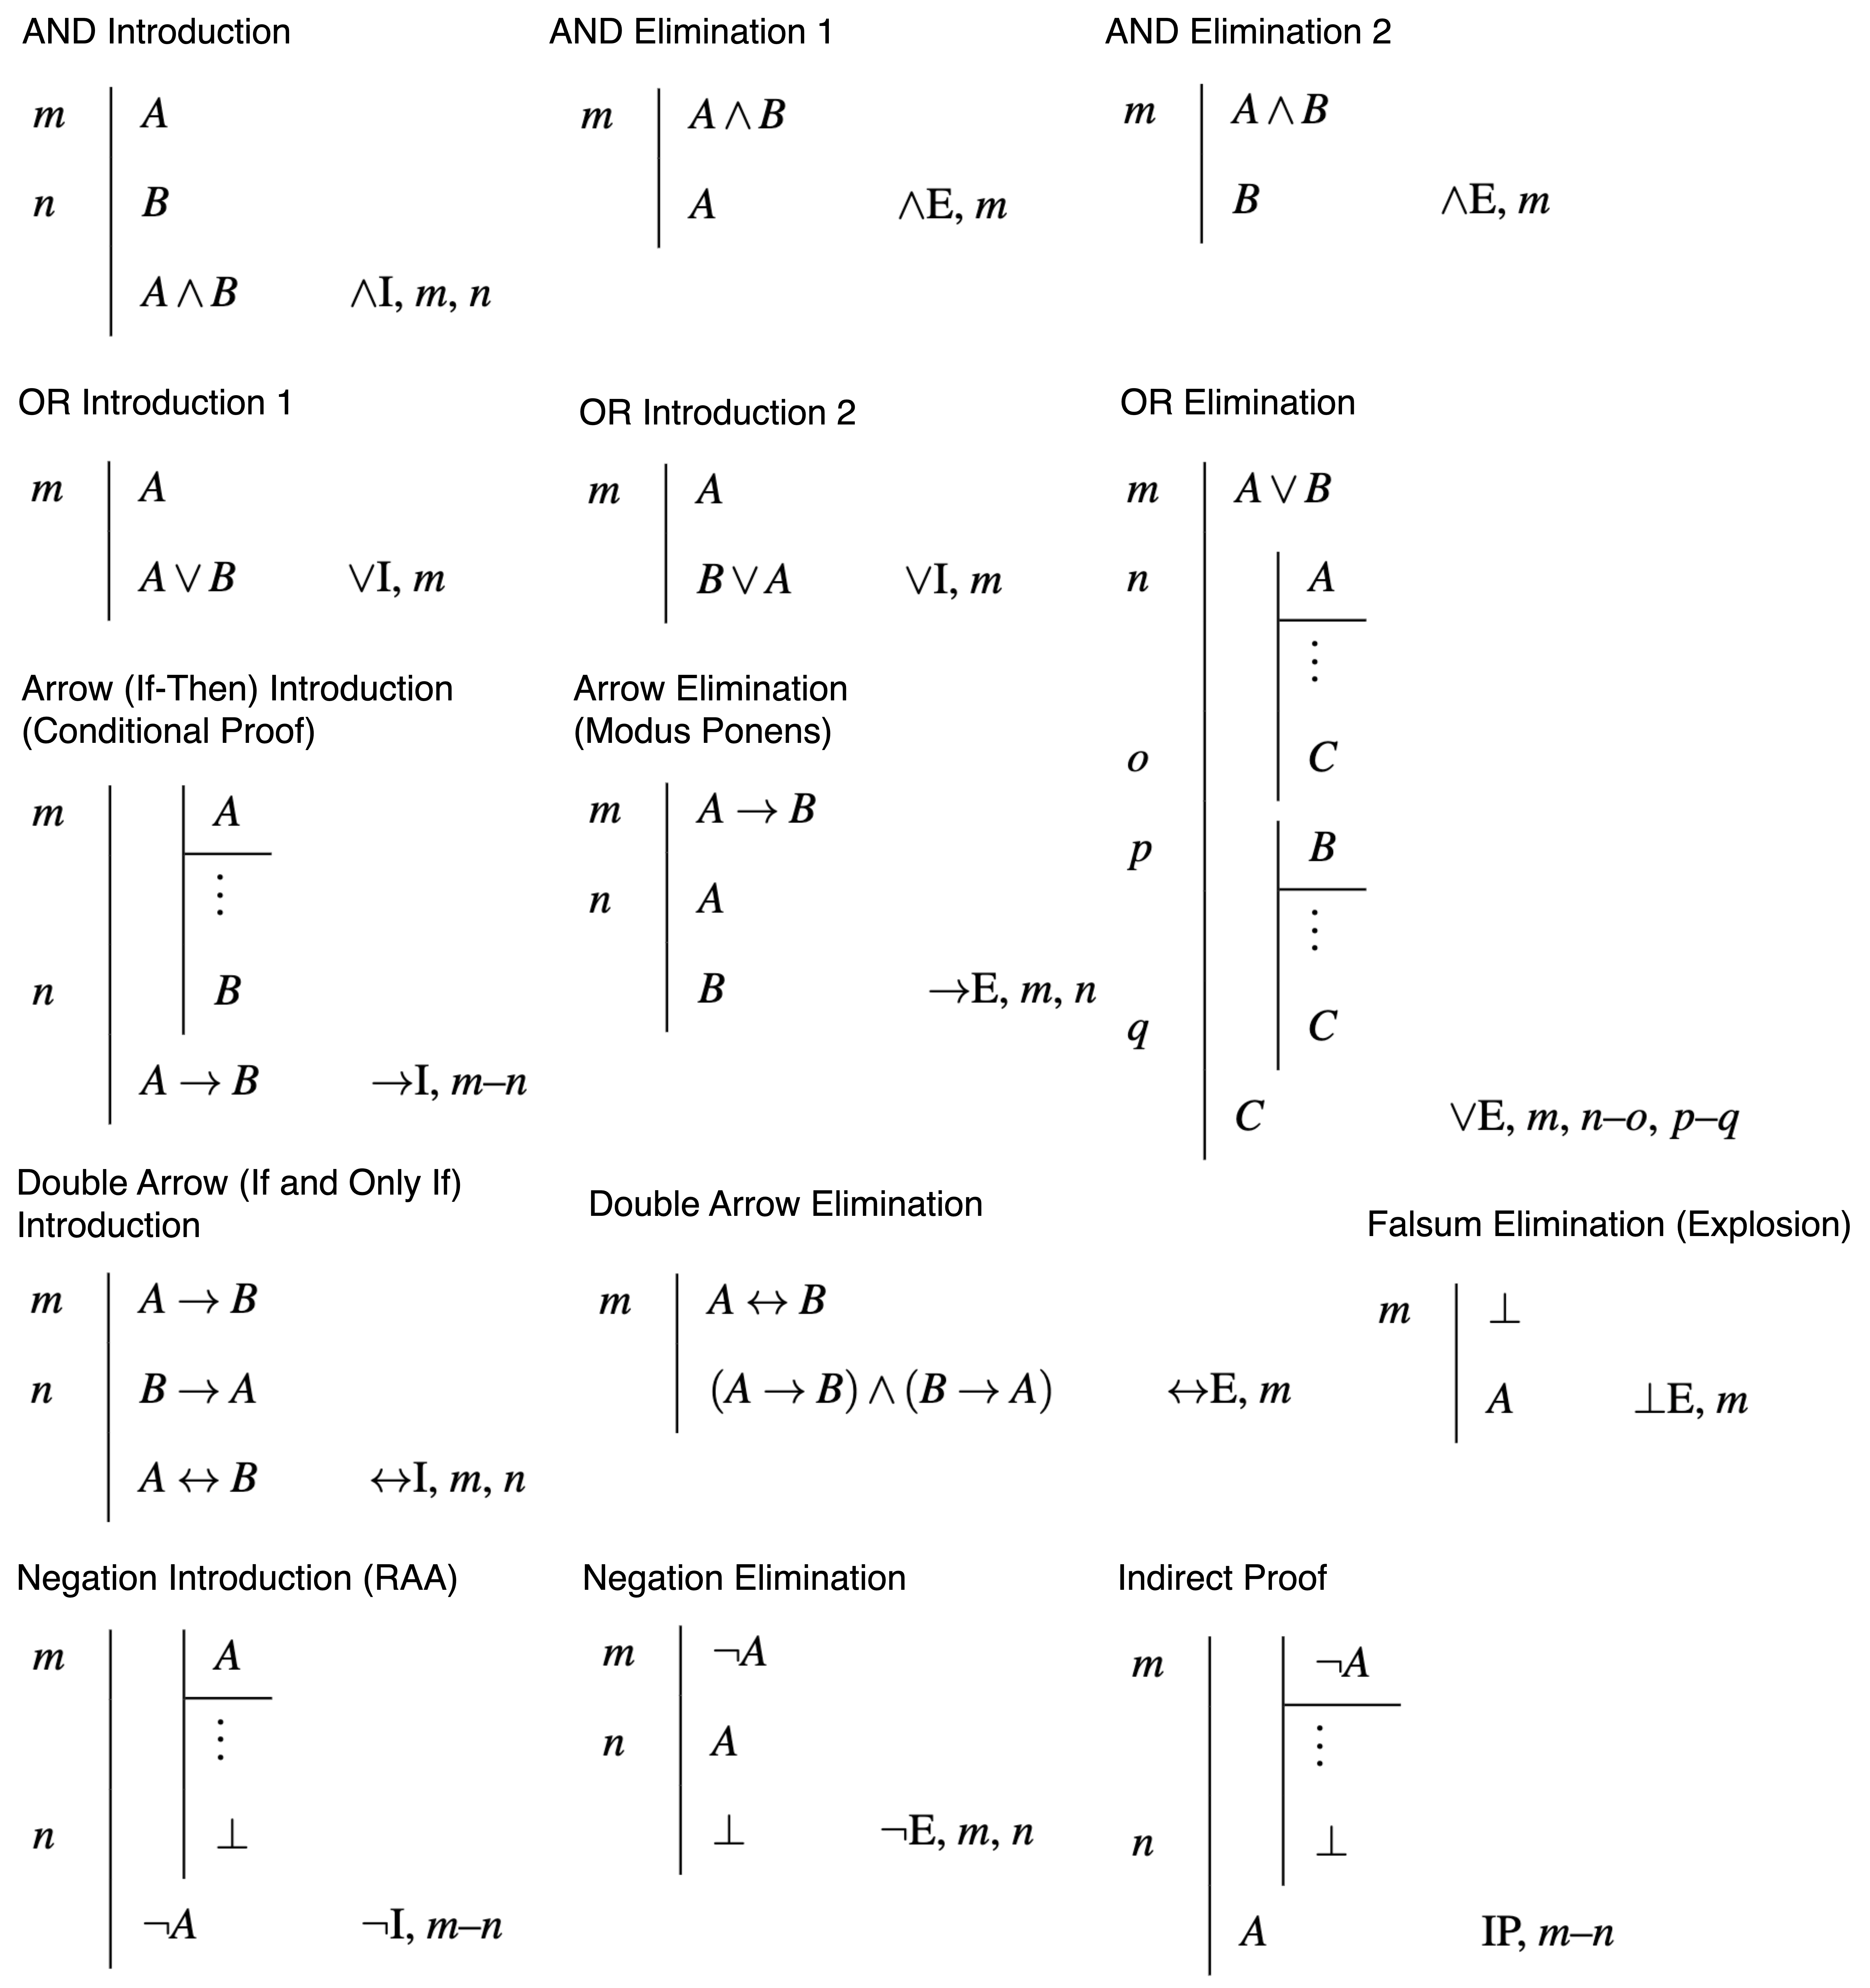
\includegraphics[width=1.1\textwidth]{Figures/Prop_rules_no_background.png}
\end{center}
These fourteen rules form Classical Propositional logic. When you include the five extra rules for Quantifiers and Identity (\ref{ssec:quant_quick}) you get First-Order logic. If you drop Indirect Proof you get Intuitionistic Propositional/First-Order Logic.
\newpage
\section{A brief word about \textit{Scope} in proofs}
We would like to take a moment to discuss scope\footnote{one might argue these are more aptly labeled ``observations on context" rather than scope.} in proofs. When applying an inference rule (i.e. an introduction or elimination rule) to justify a proof step, one can refer to proof step numbers preceeding it so long as the previous step is either in the \textit{same level of scope} (e.g. in the following proof, 11 refers to 10) or at the preeceding step numbers in any of its \textit{outer scope} layers (e.g., 10 refers 6). 

As a non-example, step 11 \textit{cannot} refer to step 8 to deduce its claim because the scope that line 8 exists in is neither the same scope as line 11 (the scope that opened at line 7 was closed at line 8 and is not the same as the scope, that opened at line 9, that line 11 is under) nor is it an outer scope of line 11 \footnote{{while the scopes of line 8 and line 11 share the same parent scope (beginning at line 6), they are \textit{independent} scopes as one closed before the other one opened, they are more like ``sibling scopes". The assumptions of these two scopes are fundamentally different: line 8 is under the assumptions introduced in lines 1, 6 and 7 whereas line 11 is under the assumptions introduced in lines 1, 6, and 9, which are not the same! }}. \\

\noindent Let's look at two proofs, which are both valid, for one of the later exercises in this doc\footnote{Exercise 6b from section \ref{subsec:PropExercises} \\ \\ \\ \\ }:

\noindent Suppose we want to show that from $(A\lor B) \wedge (A\lor C) $, $A\lor (B\wedge C)$ can be proven ( i.e. we want to show $(A\lor B) \wedge (A\lor C) \vdash A\lor (B\wedge C)$ ), well one proof (Proof A) that accomplishes this goes as follows:
$\vdash$ :
\begin{equation}
\begin{nd}
    \hypo{1}{(A \lor B) \land (A \lor C)}
    \have{2}{A \lor B} \ae{1}
    \have{3}{A \lor C} \ae{1}
    \open{}
        \hypo{4}{A}
        \have{5}{A \lor (B \land C)} \oi{4}
    \close{}
    \open{}
        \hypo{6}{B}
        \open{}
        \hypo{7}{A}
        \have{8} {A\lor (B\wedge C)} \oi{7}
        \close{}
        \open{}
            \hypo{9}{C}
            \have{10}{B \land C} \ai{6,7}
            \have{11}{A \lor (B \land C)} \oi{10}
        \close{}
        \have{12}{A \lor (B \land C)} \oe{3,7-8,9-11}
    \close{}
    \have{13}{A \lor (B \land C)} \oe{2,4-5,6-12}
\end{nd} \nonumber
\end{equation}

Here is another proof (Proof B) that uses a result at an outer scope to reduce some redundancy; note that, in the previous proof, lines 7 and 8 aren't really needed as the same lines were shown at an outer scope (lines 4 and 5) so we could just invoke 4-5 on line 12: \\

%\newgeometry{left=3cm,bottom=0.1cm}
\enlargethispage{4cm}
\hspace{-0.3in}\begin{minipage}[t]{0.45\textwidth}
New Proof (Proof B):
\begin{equation}
\begin{nd}
    \hypo{1}{(A \lor B) \land (A \lor C)}
    \have{2}{A \lor B} \ae{1}
    \have{3}{A \lor C} \ae{1}
    \open{}
        \hypo{4}{A}
        \have{5}{A \lor (B \land C)} \oi{4}
    \close{}
    \open{}
        \hypo{6}{B}
        \open{}
            \hypo{7}{C}
            \have{8}{B \land C} \ai{6,7}
            \have{9}{A \lor (B \land C)} \oi{8}
        \close{}
        \have{10}{A \lor (B \land C)} \oe{3,4-5,7-9}
    \close{}
    \have{11}{A \lor (B \land C)} \oe{2,4-5,6-10}
\end{nd} \nonumber
\end{equation}
\end{minipage}
\hspace{0.75in}
\begin{minipage}[t]{0.45\textwidth}
Old Proof (Proof A):
\begin{equation}
\begin{nd}
    \hypo{1}{(A \lor B) \land (A \lor C)}
    \have{2}{A \lor B} \ae{1}
    \have{3}{A \lor C} \ae{1}
    \open{}
        \hypo{4}{A}
        \have{5}{A \lor (B \land C)} \oi{4}
    \close{}
    \open{}
        \hypo{6}{B}
        \open{}
        \hypo{7}{A}
        \have{8} {A\lor (B\wedge C)} \oi{7}
        \close{}
        \open{}
            \hypo{9}{C}
            \have{10}{B \land C} \ai{6,7}
            \have{11}{A \lor (B \land C)} \oi{10}
        \close{}
        \have{12}{A \lor (B \land C)} \oe{3,7-8,9-11}
    \close{}
    \have{13}{A \lor (B \land C)} \oe{2,4-5,6-12}
\end{nd} \nonumber
\end{equation}
\end{minipage}
Note, in the new proof, we omit the redundant lines (lines 7 and 8 of the old proof) and instead we make reference to 4-5 in the outer scope (the scope that begins at 1 in the new proof and the old proof) to justify our ``or-elimination" on line 10.
%\restoregeometry

\section{Deriving Rules from Existing Rules}
It is often convenient to create some new rules from our existing rules so our proofs don't have to be so wordy. Let's look at a few rules that can be derived from our existing rules. Note that these new rules do not introduce any new capabilities as they are derived from the existing rules; they don't add anything new in the sense that if we can do something with these new rules, we could do it from our original rules as well, these new rules are a convenience to make our proofs a bit more compact.
\subsection{Modus Tollens }
We want to show the following:
\begin{equation}
    \begin{nd}
        \have[~]{} {A \rightarrow B}
        \have[~]{} {\neg B}
        \have[~]{} {\neg A}
    \end{nd} \nonumber
\end{equation}
That is, from the premises ``if $A$ then $B$" and ``not $B$" we can infer ``not $A$", the proof makes use of \textit{reductio ad absurdum} and looks like this:
\begin{equation}
    \begin{nd}
        \hypo{1} {A \rightarrow B}
        \hypo{2} {\neg B}
        \open{}
        \hypo{3} {A}
        \have{4} {B} \by{$\rightarrow E$ (MP)}{1,3}
        \have{5} {\bot} \ne{2,4}
        \close{}
        \have{6} {\neg A} \ni{3,5}
    \end{nd} \nonumber
\end{equation}
\subsection{Repetition}
This example seems almost too trivial to mention but there is a valid way to prove that you can re-use a statement $A$ that has already been established in the proof somewhere, the proof goes like this:
\begin{equation}
    \begin{nd}
        \hypo{1} {A}
        \have{2} {A \wedge A} \ai{1,1}
        \have{3} {A} \ae{2}
    \end{nd} \nonumber
\end{equation}

\subsection{Double Negation Elimination ($\neg\neg E$)}
\label{subsec:DNE}
Double negation elimination\footnote{ Note that since this rule relies on IP it is only valid in classical logic, not intuitionistic} is a rule that says ``not not $A$" implies $A$, we can derive it from our other rules as follows:
\begin{equation}
    \begin{nd}
        \hypo{1} {\neg \neg A}
        \open{}
        \hypo{2} {\neg A}
        \have{3} {\bot} \ne{1,2}
        \close{}
        \have{4} {A} \by{IP}{2,3}
    \end{nd} \nonumber
\end{equation}
Double negation elimination is commonly notated $\neg\neg E$
\subsection{Disjunctive Syllogism}
As we mentioned before, disjunctive syllogism is a rule that says ``Given $A\lor B$ and $\neg A$, we can infer $B$, let's look at two proofs of this, one that relies on explosion, and one that relies on indirect proof:
\begin{equation}
    \begin{nd}
        \hypo{1} {A\lor B}
        \hypo{2} {\neg A}
        \open{}
        \hypo{3} {A}
        \have{4} {\bot} \ne{2,3}
        \have{5} {B} \be{4}
        \close{}
        \open{}
        \hypo{6} {B}
        \have{7} {B} \by{Repetition}{6}
        \close{}
        \have{8} {B} \oe{1, 3-7}
    \end{nd} \nonumber
\end{equation}
Here is another approach to deriving this rule that relies on indirect proof (via DNE\footnote{ Note that since this proof relies on DNE (which relies on IP) it is only valid in classical logic, not intuitionistic})
\begin{equation}
    \begin{nd}
        \hypo{1} {A\lor B}
        \hypo{2} {\neg A}
        \open{}
        \hypo{3} {\neg B}
        \open{}
        \hypo{4} {A}
        \have{5} {\bot} \ne{2,4}
        \close{}
        \open{}
        \hypo{6} {B}
        \have{7} {\bot} \ne{3,6}
        \close{}
        \have{8}{\bot} \oe{1,4-7}
        \close{}
        \have{9}{\neg \neg B} \ni{3-8}
        \have{10} {B} \nne{9}
    \end{nd} \nonumber
\end{equation}

\section{Practice problems}
You've seen the introduction and elimination rules for classical natural deduction, now let's get some practice constructing proofs with these. To begin we will hold your hand and walk through a handful of proofs and then we will present you with the problems to tackle on your own, proofs for all problems will (eventually) be provided at the end of this document but it is highly encouraged to take a stab at each problem to get comfortable using the rules.

\subsection{Proving $p\rightarrow (q\rightarrow r) \vdash q\rightarrow (p\rightarrow r)$}
So from the premise ``if $p$ then if $q$ then $r$" we are going to derive ``if $q$ then if $p$ then $r$.
\begin{equation}
    \begin{nd}
        \hypo{1} {p\rightarrow(q\rightarrow r)}
        \open{}
        \hypo{2} {q}
        \open{}
        \hypo{3} {p}
        \have{4} {q\rightarrow r} \by{$\rightarrow E$ (MP)}{1,3}
        \have{5} {r} \by{$\rightarrow E$ (MP)}{2,4}
        \close{}
        \have{6} {p\rightarrow r} \by{$\rightarrow I$ (CP)}{3,5}
        \close{}
        \have{7} {q\rightarrow (p\rightarrow r)} \by{$\rightarrow I$ (CP)}{2,6}
    \end{nd} \nonumber
\end{equation}
So here was our strategy, we start by assuming our premise ``$p\rightarrow (q\rightarrow r)$", we wanted to arrive at ``$q\rightarrow (p\rightarrow r)$", so we want to introduce an arrow which can be done via conditional proof. So we started off by assuming the antecedent $q$ and tried to prove the consequent $(p\rightarrow r)$, then we saw we needed to introduce a new arrow so we kind of rinsed and repeated, assumed our new antecedent $p$ and tried to prove the consequent $r$. So we used conditional proof twice, one nested within the other.
\subsection{Proving $p\rightarrow (q\rightarrow r) \vdash (p\wedge q)\rightarrow r$}
This proof will go quite similarly to the previous so you might try this on your own and then have a look at this proof:
\begin{equation}
    \begin{nd}
        \hypo{1} {p\rightarrow(q\rightarrow r)}
        \open{}
        \hypo{2} {p\wedge q}
        \have{3} {p} \ae{2}
        \have{4} {q\rightarrow r} \by{$\rightarrow E$ (MP)}{1,3}
        \have{5} {q} \ae{2}
        \have{6} {r} \by{$\rightarrow E$ (MP)}{4,5}
        \close{}
        \have{7} {(p\wedge q)\rightarrow r} \by{$\rightarrow I$ (CP)}{2,6}
    \end{nd} \nonumber
\end{equation}

\subsection{Proving $p \rightarrow (q \rightarrow r) \vdash (p\rightarrow q) \rightarrow (p\rightarrow r)$}

\begin{equation}
    \begin{nd}
        \hypo{1} {p\rightarrow(q\rightarrow r)}
        \open{}
        \hypo{2} {p \rightarrow q}
        \open{}
        \hypo{3} {p}
        \have{4} {q \rightarrow r} \by{$\rightarrow E$ (MP)}{1,3}
        \have{5} q \by{$\rightarrow E$ (MP)}{2,3}
        \have{6} r \by{$\rightarrow E$ (MP)}{4,5}
        \close{}
        \have{7} {p \rightarrow r} \by{$\rightarrow I$ (CP)}{3,6}
        \close{}
        \have{8}{(p\rightarrow q)\rightarrow (p\rightarrow r)} \by{$\rightarrow I$ (CP)}{2,7}
    \end{nd} \nonumber
\end{equation}
\subsection{More practice Problems}
\label{subsec:PropExercises}
Statements of the form $A\dashv \vdash B$, can be read as ``$A$ is equivalent to $B$", so the method of proof is to show both that $B$ can be proven from $A$ and that $A$ can be proven from $B$ (i.e. two proofs).


Prove each of the following:
\begin{enumerate}
     \item $A \wedge B \dashv \vdash B \wedge A$ \hfill (Commutativity)
    \item $A \lor B \dashv \vdash B \lor A$ \hfill (Commutativity)
    \item $A \wedge (B \wedge C) \dashv \vdash (A \wedge B) \wedge C$ \hfill (Associativity)
    \item $A \lor (B \lor C) \dashv \vdash (A \lor B) \lor C$ \hfill (Associativity)
    \item $A \wedge (B \lor C) \dashv \vdash (A \wedge B) \lor (A \wedge C)$ \hfill (Distribution)
    \item $A \lor (B \wedge C) \dashv \vdash (A \lor B) \wedge (A \lor C)$ \hfill (Distribution)
    \item $\neg (A \wedge B) \dashv \vdash \neg A \lor \neg B$ \hfill (De Morgan's)
    \item $\neg (A \lor B) \dashv \vdash \neg A \wedge \neg B$ \hfill (De Morgan's)
    \item $\neg \neg A \dashv \vdash A$ \hfill (Double Negation)
    \item $A \rightarrow B \dashv \vdash \neg A \lor B$ \hfill (if-then)
    \item $A\wedge \neg B \dashv \vdash \neg (A\rightarrow B)$ \hfill (Negation of if-then)
    \item $A\rightarrow B \dashv \vdash \neg (A\wedge \neg B)$ \hfill (Another \footnote{This form shows up less often than the one from exercise \# 10, but it can be a useful way to express the arrow...} way to express if-then)
\end{enumerate}
\newpage 
\section{Introduction and Elimination Rules for Quantifiers}
We've seen how the rules for natural deduction and have gotten our feet wet with some proofs, so far the set of rules we have constitute what is known as \textit{propositional logic}, in order to get \textit{First order logic} we just need an introduction and elimination rule for each of the quantifiers: The existential quantifier $\exists$ and the universal quantifier $\forall$. Two of these rules are very straightforward, the other two require some nuance. We will start with the straightforward rules and then discuss the more nuanced ones after.

\subsection{Universal Elimination ($\forall E$)}
This rule is quite easy to understand, it basically says if ``for all $x$, $F(x)$ is true, then we can conclude $F(a)$ for a specific $a$.
\begin{equation}
    \begin{nd}
        \have{} {\forall \ x \ Fx}
        \have{} {Fa}
    \end{nd}\nonumber
\end{equation}
For example, from ``all humans are mortal" we can conclude ``I am mortal" we can conclude ``you are mortal", and so on.

The general form for this rule looks like this:
\begin{equation}
    \begin{nd}
        \have[m]{1} {\forall \ x \ A(\cdots x \cdots x \cdots)}
        \have[~]{} {A(\cdots c \cdots c \cdots)} \Ae{1}
    \end{nd}\nonumber
\end{equation}
A brief explanation of this notation: On the first line, we have some sentence $A$ that's got in it some instances of $x$ as a free variable ($A(\cdots x \cdots x \cdots)$) bound by the quantifier out front ($\forall x$), so the first line is referring to any universally quantified sentence $A$ that's got some occurrences of $x$ in it. The second line is exactly the same sentence but with all occurrences of variable $x$ replaced with some name $c$. We can keep repeating this rule with different names.

\subsection{Existential Introduction ($\exists I$)}
This rule is also quite straightforward, from ``I am sleepy" we can infer that ``someone is sleepy". Or, ``from $Fa$" we can infer ``there is an $x, Fx$"
\begin{equation}
    \begin{nd}
        \have{} {Fa}
        \have{} {\exists x Fx}
    \end{nd}\nonumber
\end{equation}
The general form of this rule looks like this:
\begin{align}
    &\begin{nd}
        \have[m]{1} {A(\cdots c \cdots c \cdots)}
        \have[~]{} {\exists x A(\cdots c \cdots x \cdots)} \Ei{1} %\by{$x$ not in $A$}{}
    \end{nd}\nonumber\\
    &x \text{ must not occur in }A \nonumber
\end{align}
Notice here we don't need to replace \textit{all} instances of $c$ with $x$ (where the $x$ is bound by the $\exists$ quantifier) we \textit{can} replace all of them but we don't have to, we might just replace some of them. So this notation could be read ``replace some or all of the $c$'s with $x$'s".

Why is it that we are allowed to replace just some of them? Well consider this example:
Suppose that we have a relation 
\begin{equation}
    Rxy = ``x \text{ trusts } y \text{ with the keys to the Lamborghini}" \nonumber
\end{equation}
 and suppose we have that ``Michael trusts himself with the keys to the Lamborghini" ($Rmm$), well from that we can infer $\exists x Rxx \ \ =$  ``someone trusts themselves with the keys", but we can also infer $\exists x Rmx \ \ =$ ``Michael trusts someone with the keys...", we can also infer $\exists x Rxm \ \ =$ ``someone trusts Michael with the keys..." and lastly, in two steps, we should be able to infer $\exists x \exists y Rxy \ \ =$ ``someone trusts someone with the keys..."

We should be able to infer all of these from ``Michael trusts himself with the keys..." ($Rmm$) so to make room for that we have to allow ourselves to replace just some of the $c$'s with $x$'s

One last thing to be careful about with existential introduction is that $x$, the variable we are introducing, isn't already in sentence $A$ as a free variable, the reason for this is: if there were an $x$ in $A$ (top line), then when we tack the existential quantifier $\exists x$ on the front (bottom line) of the sentence, it would bind the $x$ that had been free in $A$, so we would start off with an open sentence and end up with a closed sentence, which wouldn't be a valid inference. So just be careful, whenever you are using existential introduction, whatever quantifier we use ``there is an $x$" or ``there is a $z$" we have to make sure the $x$ or $z$ (or whatever new variable you choose) isn't already in $A$.

\subsection{Universal Introduction ($\forall I$)}
With universal introduction we are trying to introduce something of the form ``for all $x$, $A$" into our proof, conceptually this is a bit daunting, how can we prove that \textit{everything} is a certain way? Well lets look at two example proofs for a hint at a clever way to make such a leap. We will present one proof with good reasoning and another with faulty reasoning and examine their differences.

\textbf{Good reasoning: }
Suppose we start off by assuming that $a$ is $F$ and from that we infer $a$ is $F$ or $G$. From that we can conclude from arrow introduction (CP) that ``if $a$ is $F$ then it's $F$ or $G$", and from that we can conclude that \textit{everything} is such that ``if it's $F$ then it's $F$ or $G$"
\begin{equation}
    \begin{nd}
    \open{}
        \hypo{} {Fa}
        \have{} {Fa \lor Ga}
        \close{}
        \have{} {Fa \rightarrow (Fa\lor Ga)}
        \have{} {\forall x (Fx \rightarrow (Fx \lor Gx))}
    \end{nd}\nonumber
\end{equation}
Now let's look at something that looks quite similar but is bad reasoning

\textbf{Bad Reasoning:}
Suppose we start off with a premise that $a$ is $F$, and then we assume further than $a$ is also $G$, we can conclude that $a$ is both $F$ and $G$, then using arrow introduction we can infer if $a$ is $G$ then $a$ is $F$ and $G$, now suppose we try to make the same move that we made in the last example, inferring that this line ($Ga \rightarrow (Fa\wedge Ga)$) applies to everything... i.e. we attempt to conclude that \textit{everything} is such that if its $G$ then it's $F$ and $G$. That's obviously not correct, just because something is $G$ doesn't mean that it's both $F$ and $G$ in general.
\begin{equation}
    \begin{nd}
        \have{} {Fa}
        \open{}
        \hypo{} {Ga}
        \have{} {Fa \wedge Ga}
        \close{}
        \have{} {Ga \rightarrow (Fa \wedge Ga)}
        \have{} {\forall x (Gx \rightarrow (Fx \wedge Gx))} \by{THIS STEP IS NOT VALID!}{}
    \end{nd}\nonumber
\end{equation}

So that first example was good reasoning and the second was bad but what was the difference? Well, the difference is how the name $a$ is used in these two proofs. In the second proof, the bad proof, we had some information about $a$, we then assumed something further about $a$, inferred some stuff, and then concluded that everything is like that, well that just doesn't make sense, because our premise was about a specific $a$, we can't generalize from a specific thing to a general fact. Suppose $F(x)=``x$ is American" and $G(x)=``x$ has no pets", then in this second proof we are saying something like: Jack is American, now suppose Jack also has no pets, then Jack is American and Jack has no pets, so if Jack has no pets then Jack is American and has no pets, we can't suddenly leap to the conclusion that for any individual if they have no pets then they are American and have no pets! You can't go from specific information about someone to inferring it applies to everyone. 

In the first proof on the other hand, we don't start off with specific information about anyone/anything, at the top we start off with nothing, then we make an assumption about a random person/thing $a$, who or what is $a$? They are arbitrary, they don't appear in the proof before so it is an \textit{arbitrary name} (it doesn't appear in the proof up to this point \footnote{Technically an \textit{arbitrary} name \textit{can} appear in the proof before, the exact criteria is: it can't appear in any undischarged assumption or premise.}) and we haven't got any prior information about this $a$. So what we did is first we cooked up this arbitrary name $a$, we say suppose $a$ is American, then $a$ is American or they have no pets, then we introduce the arrow if $a$ is American then $a$ is American or $a$ has no pets, and since $a$ is not a specific individual, it's an arbitrary individual, we can infer that everyone's like that.

This is the key point for universal introduction: we first show it's the case for an arbitrary name and then we can infer it's the case for all names.


Ok now for the actual introduction rule for universal quantifier:
If you can infer that $A$ holds for an arbitrary name $c$ then you can infer from that that it holds for all names.
\begin{align}
    &\begin{nd}
        \have[m]{1} {A(\cdots c \cdots c \cdots)} 
        \have[~]{} {\forall x A(\cdots x \cdots x \cdots)} \Ai{1} 
    \end{nd}\nonumber \\
    &c \text{ arbitrary (not in an undischarged assumption)} \nonumber \\
    &x \text{ not in }A \nonumber
\end{align}
This is the introduction rule for the universal quantifier ($\forall I$). \\

The reader should note that $c$ being \textit{arbitrary} and $x$ not appearing in $A$ are part of the rule! Some authors use a convention known as flagging to indicate when an arbitrary name like $c$ has been introduced into the proof for the purpose of universal introduction. This approach is typicaly required when using a proof verifier as the act of ``flagging" the arbitrary name allows the verifier to run back through your proof to ensure you haven't used it before. With this convention, the introduction rule for the universal quantifier looks like this:
\begin{align}
    &\begin{nd}
    \open{}
    \hypo[m]{1} {c} \by{Flag}{}
    \have[~]{}{\vdots}
        \have[n]{2} {A(\cdots c \cdots c \cdots)} \by{}{}
        \close{}
        \have[~]{} {\forall x A(\cdots x \cdots x \cdots)} \Ai{1-2}
    \end{nd}\nonumber\\
    &x \text{ not in } A \nonumber
\end{align}
\subsection{Existential Elimination Rule ($\exists E$)}
Suppose we know $\exists x Fx$ and we know that $\forall x (Fx \rightarrow Gb)$ then you can infer $Gb$
\begin{equation}
    \begin{nd}
        \have{} {\exists x Fx}
        \have{} {\forall x (Fx\rightarrow Gb)}
        \have{} {Gb}
    \end{nd} \nonumber
\end{equation}
Now think about how we might derive the middle sentence ($\forall x (Fx \rightarrow Gb)$), it's a universal sentence so we would have to use universal introduction like we just did in the previous section... We would start with $\exists x Fx$, we would assume $Fa$, try to derive $Gb$, then we can infer $Gb$
\begin{equation}
    \begin{nd}
        \have{} {\exists x Fx}
        \open{}
        \hypo{} {Fa}
        \have{} {Gb}
        \close{}
        \have{} {Gb}
    \end{nd} \nonumber
\end{equation}
Now for this to be good reasoning we would have to ensure that $a$ is an arbitrary name. This pattern gives us the form we are going to use for existential elimination: If we start off with the assumption that something is $F$, and then we assume that $a$ (arbitrary name) is $F$, then whatever we can infer from that, we can infer from $\exists x Fx$ provided that we dont get information about the arbitrary individual $a$ into our conclusion $Gb$. The conclusion we draw $Gb$ cannot be information about the arbitrary individual that we introduced... If we could do that we could go
\begin{equation}
    \begin{nd}
        \have{} {\exists x Fx}
        \open{}
        \hypo{} {Fa}
        \have{} {Fa} \by{ THIS IS NOT ALLOWED! }{}
        \close{}
        \have{} {Fa}
    \end{nd} \nonumber
\end{equation}
That would allow us to go from ``there is an $x$, $Fx$" to $Fa$, but then that final $Fa$ wouldn't be an arbitrary individual (we only use those in assumptions) 

The key thing we learned from this inference is that whatever we work out on line 3 ($Gb$) it can't be involving the arbitrary individual $a$.\\

\noindent Now to formulate this as a general rule:
\begin{align}
    &\begin{nd}
        \have[m]{1} {\exists x A(\cdots x \cdots x \cdots)} 
        \open{}
        \hypo[n]{2} {A(\cdots c \cdots c \cdots)} 
        \have[~]{}{\vdots}
        \have[o]{3} {B} 
        \close{}
        \have[~]{} {B} \Ee{1,2-3}
    \end{nd} \nonumber \\
    & c \text{ is arbitrary (not in any previous undischarged assumption)} \nonumber \\
    & \text{and }c \text{ not in }A(\cdots x \cdots x \cdots ) \text{ or }B \nonumber
\end{align}
This is the elimination rule for the existential quantifier ($\exists E$). 

\section{Examples with Quantifier Intro and Elim}
Let's get some practice with these new introduction and elimination rules, we will try to focus on the tricky ones to begin with. I encourage you to try them yourself first before reading the supplied proof.

\subsection{Example practising Existential Elimination}
Prove $\exists x (Fx\wedge Gx) \vdash \exists x Fx \wedge \exists x Gx$ \vspace{0.1in} \\ %(Note, the left side cannot be proven from the right, can you explain why?)\\
So the strategy for this proof will be to apply existential elimination, and ultimately we want the ``$B$" that pops out from that existential elimination to be the conjunction $\exists x Fx \wedge \exists x Gx$, so we will start with an arbitrary name $c$ and assume $Fc\wedge Gc$ and try to deduce that conjunction...
\vspace{-0.2in}
\begin{equation}
    \begin{nd}
        \hypo{1} {\exists x (Fx \wedge Gx)}
        \open{}
        \hypo{2} {Fc \wedge Gc}
        \have{3} {Fc} \ae{2}
        \have{4} {Gc} \ae{2}
        \have{5} {\exists x Fx} \Ei{3}
        \have{6} {\exists x Gx} \Ei{4}
        \have{7} {\exists x Fx \wedge \exists x Gx} \ai{5,6}
        \close{}
        \have{8} {\exists x Fx \wedge \exists x Gx} \Ee{2-7}
    \end{nd}\nonumber
\end{equation}
\newpage
\subsection{Example practising Universal Introduction}
Prove $\exists x Fx \rightarrow Ga \vdash \forall x(Fx\rightarrow Ga)$ \vspace{0.1in} \\
So what is this saying? It says if there is some $x$ such that $Fx$, then it follows that $Ga$, intuitively this should imply that for every $x$ if it is $Fx$ then $Ga$, let's work our way through using universal introduction, we will show that an arbitrary name has the property so all names have it:
\begin{equation}
    \begin{nd}
        \hypo{1}{\exists x Fx \rightarrow Ga}
        \open{}
        \hypo{2}{Fc} 
        \have{3} {\exists x Fx} \Ei{2}
        \have{4} {Ga} \by{$\rightarrow E$ (MP)}{1,3}
        \close{}
        \have{5} {Fc\rightarrow Ga} \by{$\rightarrow I$ (CP)}{2,4}
        \have{6} {\forall x (Fx\rightarrow Ga)} \Ai{5}
    \end{nd}\nonumber
\end{equation}

\subsection{More practice with quantifier rules}
\label{subsec:QuantifiersExercises}
Prove each of the following:
\begin{enumerate}
     \item $\exists x (Fx\lor Gx) \dashv \vdash \exists x Fx \lor \exists x Gx$ \hfill (Distribution of Existential Quantifier)
     \item $\neg (\exists x Fx) \dashv\vdash \forall x \neg Fx$ \hfill (Negation of Existential Quantifier)
     \item $\neg (\forall x Fx) \dashv \vdash \exists x \neg Fx$ \hfill (Negation of Universal Quantifier)
     \item $(\forall x (Px\rightarrow Qx)), \ \  (\exists x Px) \vdash \exists x Qx$
     \item $(\exists x(Bx\rightarrow Cx)), \ \ (\forall x (Cx\rightarrow Dx))\vdash \exists x(Bx\rightarrow Dx)$
     \item $(\forall x (Jx\lor Kx)), \ \  (\forall x \neg Kx) \vdash \forall x Jx$
     \item $\forall x \forall y Rxy \vdash \forall y \forall x Rxy$
     \item $\forall x (\exists yRxy \rightarrow \forall y Ryx), \ \ Rab \ \vdash \forall x \forall y Rxy$ \footnote{This is quite a tricky problem, you will need to invoke the first of these assumptions twice and take a similar approach to the previous problem for introducing the two for-alls}
\end{enumerate}
\newpage
\section{Introduction and Elimination Rules for Identity}
While some introductory logic texts forego a discussion of rules for identity ($=$) altogether, for the sake of completeness, we will discuss another set of rules that are commonly considered in treatments of first-order (predicate) logics: the rules governing the introduction and elimination of identity in natural deduction proofs.

This section is largely drawn from Rob Trueman's version of \href{https://www.rtrueman.com/forallx.html}{\texttt{forall}$\chi$}, if you are interested in a discussion of the more philosophical considerations of identity in logic (e.g. the principle known as \textit{Identity of Indiscernibles}) then feel free to read section 32 of Trueman's book. For our purposes we will simply look at the rules themselves and present the same exercises provided by Trueman.
\subsection{Identity Introduction Rule ($=$I)}
In logic we are always guaranteed that every object is identical \textit{to itself}, no premises are required to conclude $a=a$, this is our introduction rule for identity:
\begin{equation}
    \begin{nd}
        \have[~]{} {a=a} \by{=I}{}
    \end{nd} \nonumber
\end{equation}
Note that this rule does not require reference to any prior lines of the proof. For any name $a$, you can write $a = a$ at any point, with only the $=I$ rule as justification. Pretty straightforward but not all that interesting, the elimination rule is a little more interesting...

\subsection{Identity Elimination Rule ($=$E)}
Suppose you have established $a = b$. In that case, you can take any sentence with the name $a$ in it, and replace some or all of the occurrences of $a$ with the name $b$. For example, from $Raa$ and $a = b$, you are justified in inferring $Rab$, $Rba$ or $Rbb$. More generally:
\begin{equation}
    \begin{nd}
        \have[m]{1}{a=b} 
        \have[n]{2}{A(\cdots a \cdots a \cdots)}
        \have[~]{3}{A(\cdots b \cdots a \cdots)} \by{$=$E}{1,2}
    \end{nd} \nonumber
\end{equation}
The notation here is as for $\exists$I. That is, $A(\cdots a \cdots a \cdots)$ is a formula containing the name $a$, and $A(\cdots b \cdots a \cdots)$ is a formula obtained by replacing one or more instances of the name $a$ with the name $b$. Lines $m$ and $n$ can occur in either order, and do not need to be adjacent, but we always cite the statement of identity first. Symmetrically, we allow:
\begin{equation}
    \begin{nd}
        \have[m]{1}{a=b} 
        \have[n]{2}{A(\cdots b \cdots b \cdots)}
        \have[~]{3}{A(\cdots a \cdots b \cdots)} \by{$=$E}{1,2}
    \end{nd} \nonumber
\end{equation}
\subsection{An example using these rules}
Suppose we are tasked with proving the following:
\begin{align}
    \forall x (x=a\rightarrow Fx), \ b=a \ \vdash \ Fb \nonumber
\end{align}
What is this saying? Our premises are 1) for all $x$ in our universe of discourse we have that if $x$ equals $a$ then $x$ is (exhibits) $F$, and 2) $b$ equals $a$, from this we wish to prove that $b$ is $F$. Intuitively this should be true, if being equal to $a$ means you exhibit $F$ then $b$ being equal to $a$ should guarantee $b$ exhibits $F$. Our proof goes like this:
\begin{equation}
    \begin{nd}
    \hypo{1} {\forall x (x=a\rightarrow Fx)}
    \hypo{2} {b=a}
    \have{3} {a=a\rightarrow Fa} \by{$\forall$E}{1}
    \have{4} {a=a} \by{$=$I}{}
    \have{5} {Fa} \by{$\rightarrow$E}{3,4}
    \have{6} {Fb} \by{$=$E}{2,5}
    \end{nd} \nonumber
\end{equation}
\subsection{Practice problems for Identity Rules}
\label{subsec:IdentityExercises}
\begin{enumerate}
    \item $Pa \lor Qb, Qb \to b = c, \neg Pa \vdash Qc$
    \item $m = n \lor n = o, An \vdash Am \lor Ao$
    \item $\forall x \ x = m, Rma \vdash \exists x Rxx$
    \item $\forall x \forall y (Rxy \rightarrow x = y) \vdash R{ab} \to R{ba}$
    \item $\neg \exists x \, \neg x = m \vdash \forall x \forall y (Px \to Py)$
    \item $\exists x Jx, \exists x \neg Jx \vdash \exists x \exists y \, \neg x = y$
    \item $\forall x (x = n \leftrightarrow Mx), \forall x (Ox \lor \neg Mx) \vdash On$
    \item $\exists x Dx, \forall x (x = p \leftrightarrow Dx) \vdash Dp$
    \item $\exists x [(Kx \wedge \forall y (Ky \to x = y)) \wedge Bx], Kd \vdash Bd$
    \item $\vdash P_a \to \forall x (P_x \lor \neg x = a)$
\end{enumerate}
\newpage
\begin{center}
    \subsection{Quick Reference for Quantifier and Identity Intro and Elim Rules} \vspace{0.3in}
    \label{ssec:quant_quick}
    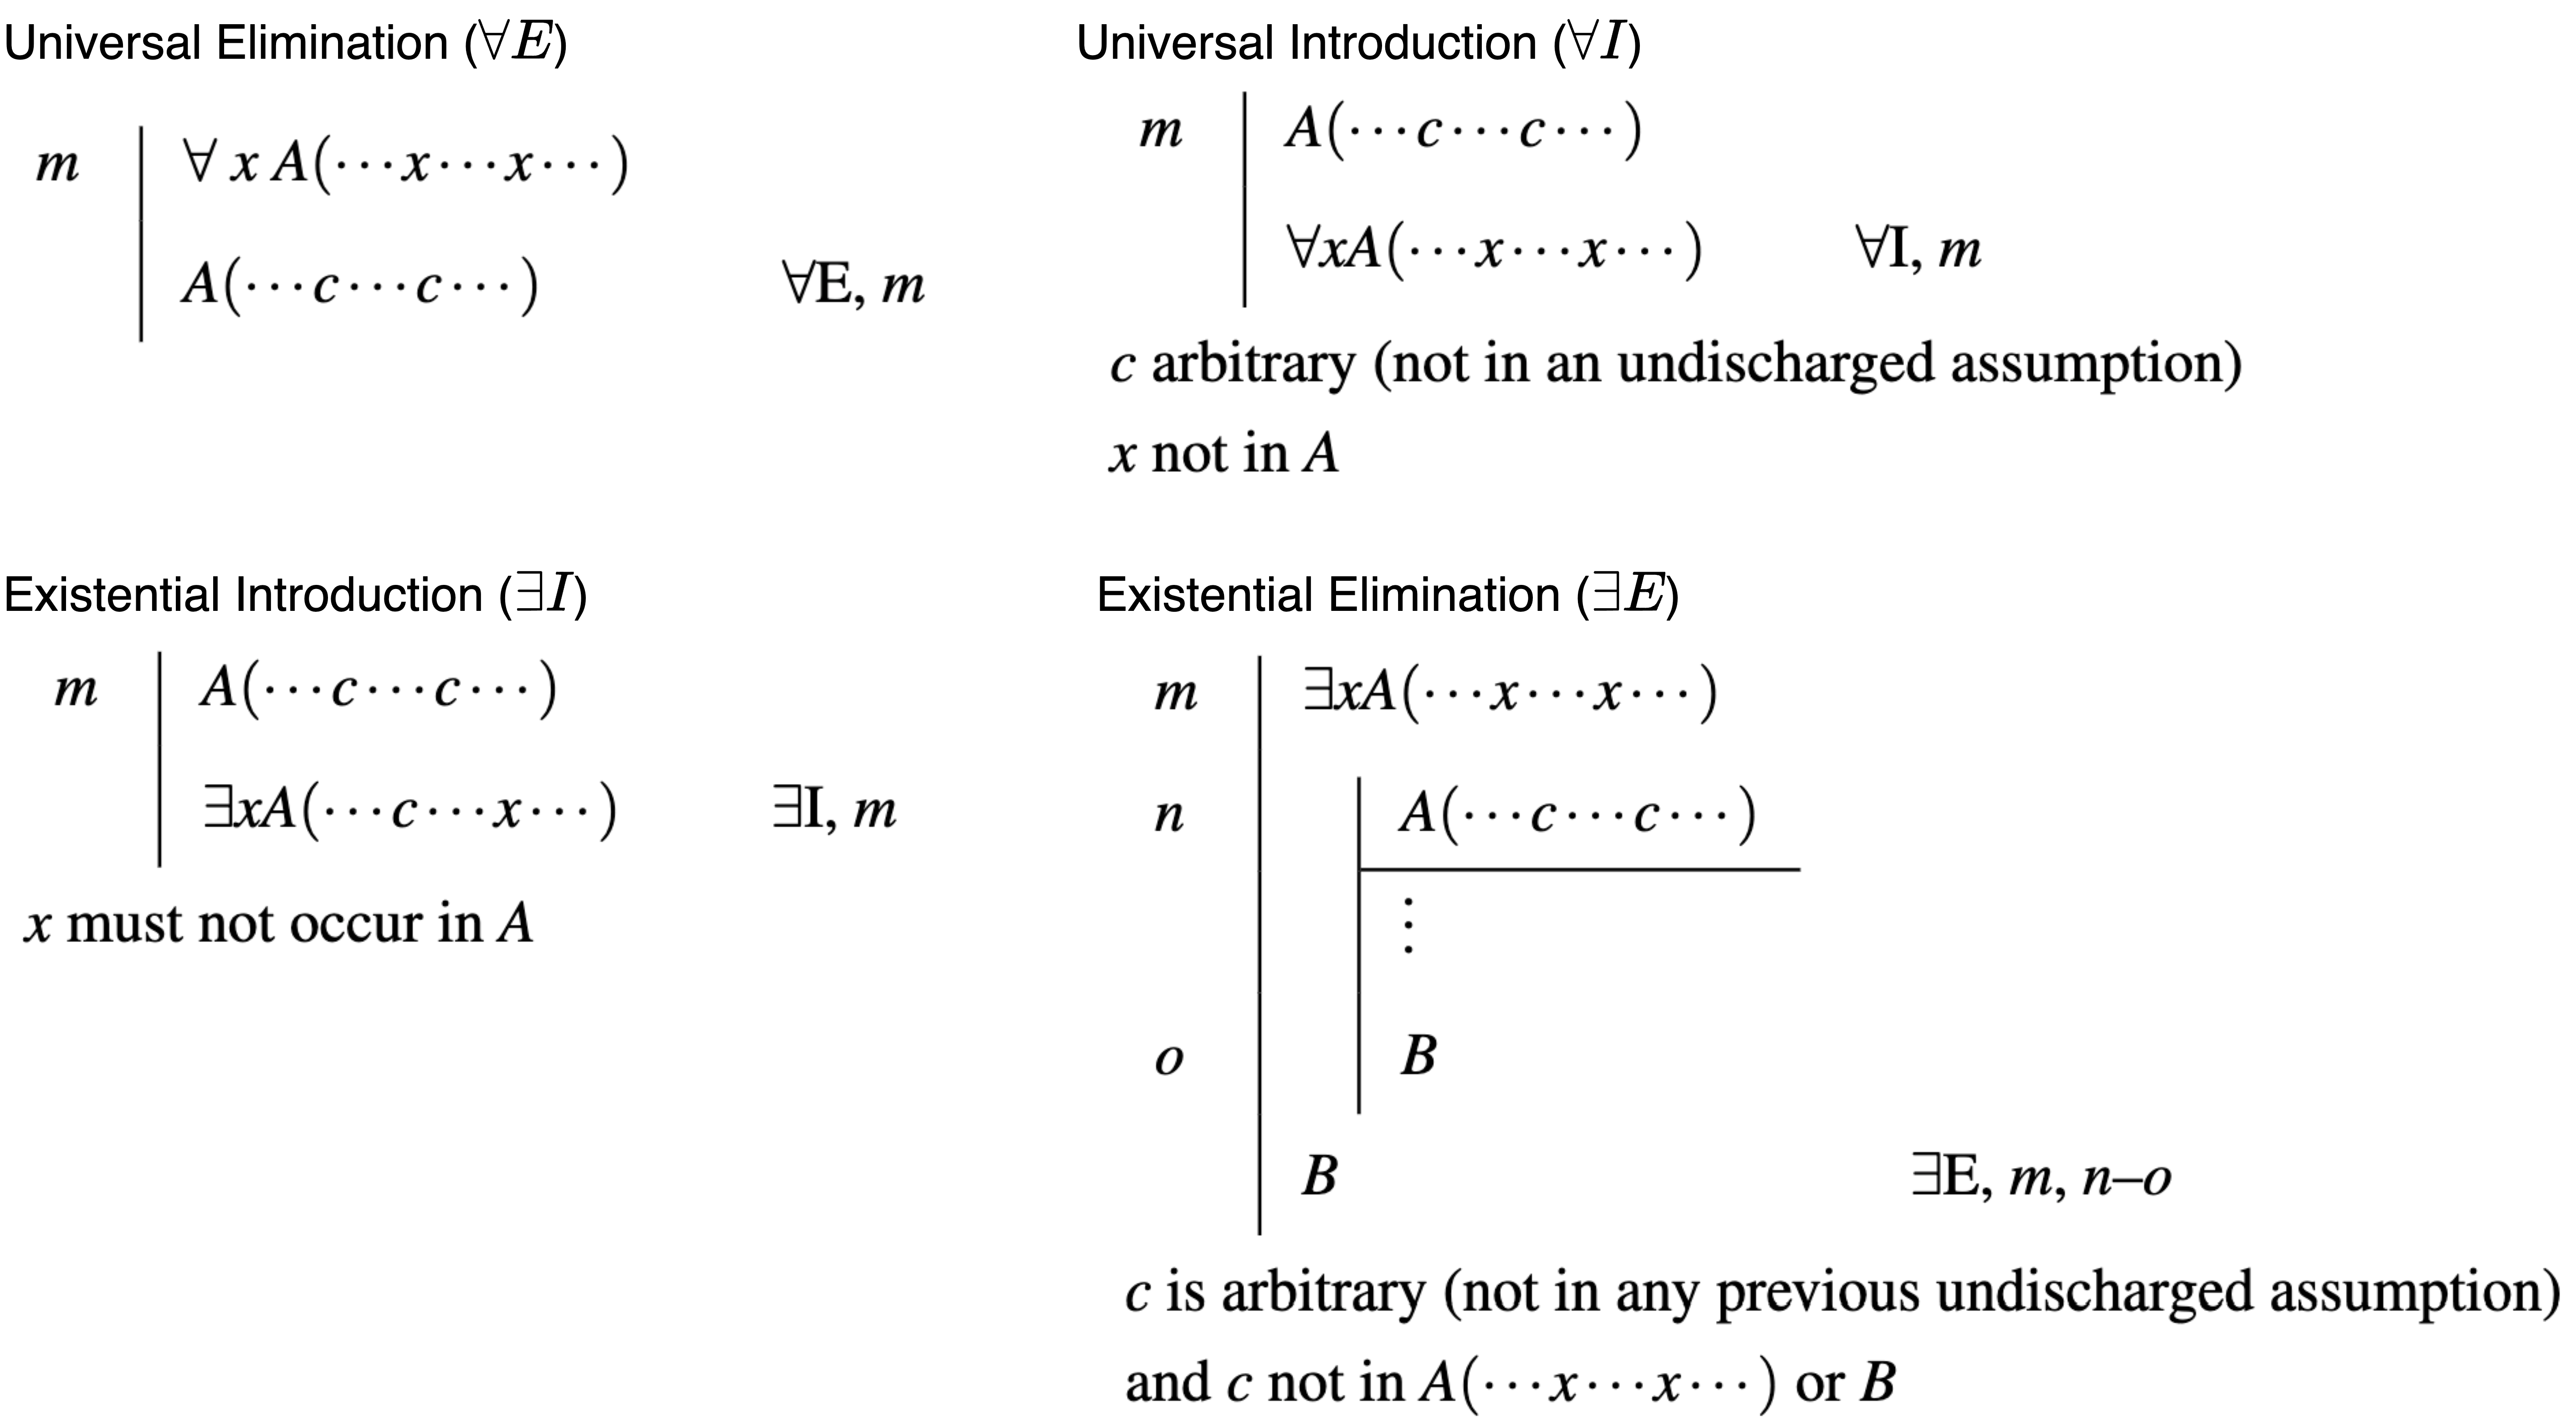
\includegraphics[width=1.1\textwidth]{Figures/Quant_rules_no_background.png} \\  \vspace{0.3in} \steezybreak 
    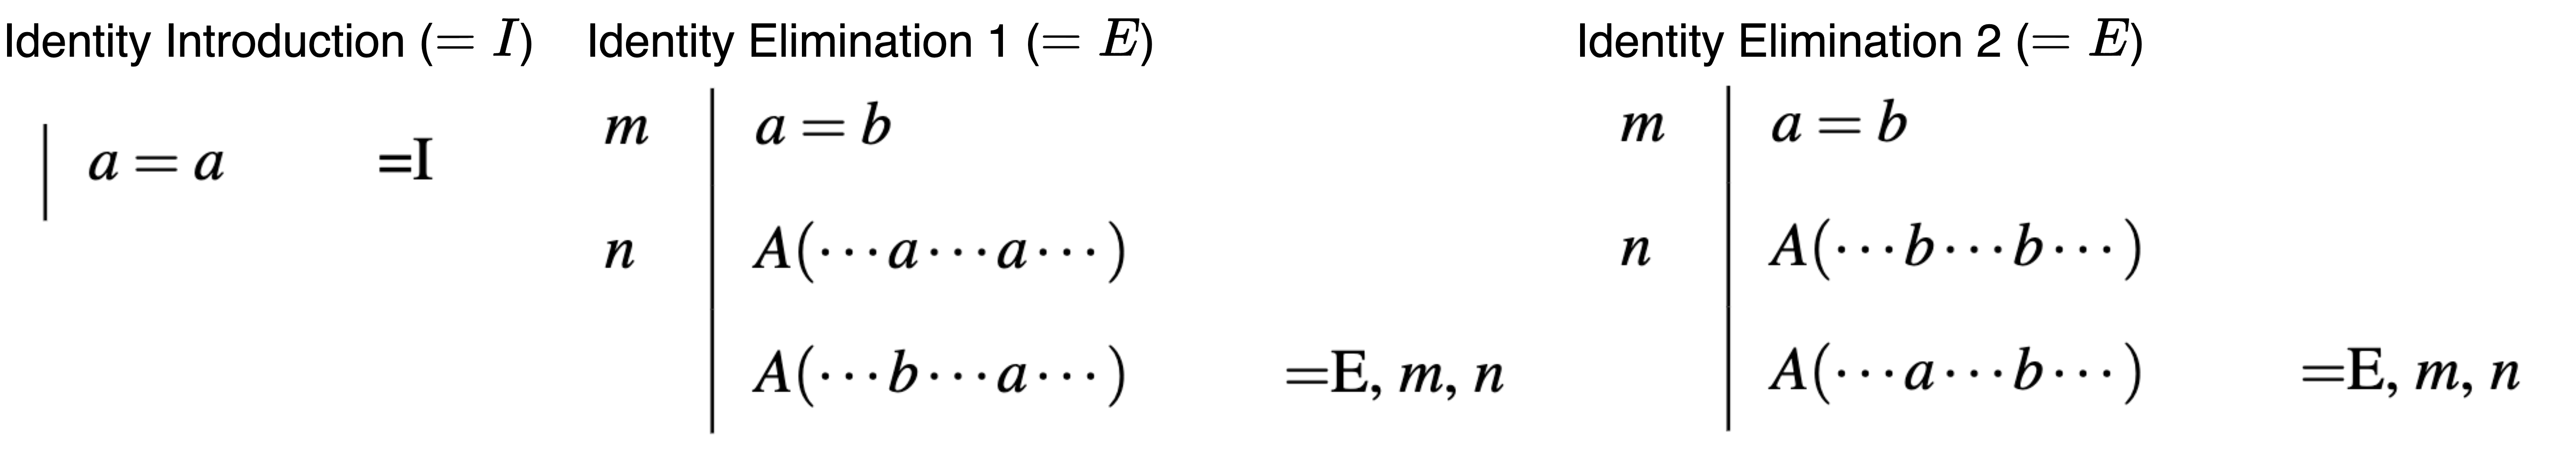
\includegraphics[width=1.1\textwidth]{Figures/Identity_rules_no_background.png} \\ \steezybreak
    These five rules, along with the fourteen rules for Propositional logic (\ref{ssec:prop_quick}) form the rules for First-Order logic.
\end{center}
\newpage
\section{A Brief Discussion on Classical vs. Intuitionistic Logic}
In the simplest terms, intuitionistic logic is classical logic \textit{without} indirect proof! Keep all the other introduction and elimination rules and do away with indirect proof (IP) and you have intuitionistic logic. Just keep this in the back of your mind and we will discuss some consequences of this.

% \subsection{Truth and Proof}

% \begin{itemize}
%     \item \textbf{Classical Logic}: Truth is often considered in a more abstract sense, independent of our ability to prove it. A statement is either true or false, regardless of whether we can prove it.
%     \item \textbf{Intuitionistic Logic}: Truth is tied to proof. A statement is only true if we can constructively prove it. The focus is on the constructive process of proving statements rather than on an abstract notion of truth.
% \end{itemize}

\subsection{Law of The Excluded Middle}
Law of the excluded middle states that for any statement $P$, either $P$ is true, or $\neg P$ is true and it is sometimes taken as an alternative axiom to IP in classical logic and is written as $P \lor \neg P$. You may have read that Intuitionism is characterized by their rejection of \textit{Law of the Excluded Middle} (LOTEM). This is true and in-fact it is equivalent to rejecting indirect proof, we will outline two arguments below that show if you have one you have the other (each can be derived from the other):

\subsubsection*{From Indirect Proof (IP) to the Law of Excluded Middle (LEM)}

Suppose we accept indirect proof. We can prove the Law of Excluded Middle as follows:

\begin{equation}
    \begin{nd}
        \hypo{1} { \ \ IP \ \ }
        \open{}
        \hypo{2} {\neg(P\lor \neg P)}
        \open{}
        \hypo{3} {P}
        \have{4} {P\lor \neg P} \oi{3}
        \have{5} {\bot} \ne{2,4}
        \close{}
        \have{6} {\neg P} \ni{3-5}
        \have{7} {P\lor \neg P} \oi{6}
        \have{8} {\bot} \ne{2,7}
        \close{}
        \have{9} {P\lor \neg P} \by{IP}{2,8}
    \end{nd}\nonumber
\end{equation}
% \begin{align*}
% 1. & \ \text{Assume } \neg (P \lor \neg P). \ \text{(Suppose that neither } P \text{ nor } \neg P \text{ is true.)} \\
% 2. & \ \text{Now further, assume } P \text{ from that we can introduce $P\lor \neg P$ and introduce $\bot$} \\
% 3. & \ \text{Then by RAA } \neg P \text{ must be true.} \\
% 4. & \ \text{But if } \neg P \text{ is true, then } P \lor \neg P \text{ must be true.} \\
% 5. & \ \text{This is a contradiction because we assumed } \neg (P \lor \neg P). \\
% 6. & \ \text{Therefore, by indirect proof, } \neg (P \lor \neg P) \text{ is false, which means } P \lor \neg P \text{ is true.}
% \end{align*}

Thus, if we accept indirect proof (IP), we can derive the Law of Excluded Middle (LEM).

\subsubsection*{From the Law of Excluded Middle (LEM) to Indirect Proof (IP)}

Conversely, if we assume the Law of Excluded Middle, we can justify indirect proof as follows \footnote{This one is a little trickier to follow because we encode the assumptions of IP as $(\neg A \rightarrow \bot)$ and want to show that when such a scenario arises, LEM allows us to come to the same conclusion that IP does}:

\begin{equation}
    \begin{nd}
        \hypo{1} {A\lor \neg A}
        \hypo{2} {\neg A \rightarrow \bot}
        \open{}
        \hypo{3} {A}
        \have{4} {A} \by{Rep.}{3}
        \close{}
        \open{}
        \hypo{5} {\neg A} 
        \have{6} {\bot} \by{$\rightarrow E$ (MP)}{2,5}
        \have{7} {A} \be{6}
        \close{}
        \have{8} {A} \oe{1, 3-4, 5-7}
    \end{nd}\nonumber
\end{equation}

% \begin{align*}
% 1. & \ \text{To prove a statement } P \text{ by contradiction, assume } \neg P \text{ and show that this assumption leads to a contradiction.} \\
% 2. & \ \text{If } \neg P \text{ leads to a contradiction, then } \neg P \text{ cannot be true, so } \neg \neg P \text{ must be true.} \\
% 3. & \ \text{By the Law of Excluded Middle, } P \lor \neg P \text{ is true.} \\
% 4. & \ \text{Since } \neg P \text{ leads to a contradiction, the only remaining possibility is that } P \text{ is true.}
% \end{align*}

Thus, if we accept the Law of Excluded Middle, we can justify indirect proof.

\begin{itemize}
    \item Intuitionistic logic does not accept the Law of Excluded Middle (LEM) as a general principle because it requires a constructive proof of \( P \) or \( \neg P \).
    \item Similarly, intuitionistic logic does not accept indirect proof because it does not consider \( \neg \neg P \) to be equivalent to \( P \); that is, showing that \( \neg P \) leads to a contradiction is not enough to conclude that \( P \) is true.
\end{itemize}

\subsection{Logical Connectives}
In Classical Logic, logical connectives such as conjunction ($\wedge$), disjunction ($\lor$), and implication ($\rightarrow$) behave according to traditional truth tables. \\

\noindent In Intuitionistic Logic: The interpretation of logical connectives is more constructive. For example, to prove $P\rightarrow Q$, one must provide a construction that converts any proof of $P$ into a proof of $Q$, in a similar vein while $\neg A \lor B \vdash A\rightarrow B$, we do not have $A\rightarrow B \vdash \neg A \lor B$ (just try to prove that direction without IP!)\footnote{Attempting to prove this other direction without IP will make you wonder, ``how can I ascertain anything about the truth values of arbitrary $A$ or $B$ from an arbitrary conditional!?" and you're right! without a tool like indirect proof it is (as far as I know) impossible! You're starting to think like an intuitionist/constructive logician!}

\subsection{Double Negation Elimination}
In classical logic, double negation is equivalent to the original statement\footnote{This was exercise 9 from Section \ref{subsec:PropExercises}}. That is, $\neg \neg P$ is logically equivalent to $P$. \\

\noindent In intuitionistic logic, $\neg \neg P$ does not necessarily imply $P$. The double negation only tells us that 
$P$ cannot be false, but it does not constructively prove $P$.

In fact a good exercise is to show that IP and DNE can be derived from one another. We actually already showed one direction of this exercise in section \ref{subsec:DNE}.
\newpage 
\section{Second Order Logic}
Alright, ngl, I'm in over my head for this section (and the last one) but I will do my best and I will be HEAVILY leaning on the work of \href{https://www.rtrueman.com/}{Dr. Rob Trueman}, in particular his extension/primer of his \texttt{forall}$\chi$ which deals with second-order logic \cite{truemanSOL}.

Dr. Trueman begins his primer by pointing out two perfectly reasonable natural language arguments, one of which can be proven with the tools of First-Order Logic alone, and the second of which requires something more. He begins like this:

\begin{tcolorbox}
    \textbf{Excerpt from \cite{truemanSOL}:}\\
    Here is a good, natural language argument:
\begin{align*}
    &\text{Bertrand is a logician}\\
    &\text{Bertrand is a mathematician}\\
    &\therefore \text{ Someone is both a logician and a mathematician}\\
\end{align*}
Here is another good, natural language argument:
\begin{align*}
   &\text{Bertrand is a philosopher}\\
   &\text{Alfred is a philosopher}\\
   &\therefore \text{ Bertrand and Alfred have something in common} \\
\end{align*}
But while both of these are perfectly good arguments, the formal tools you have been given deal only with the first, not the second. As you all know, you can formalise the first argument like this:
\begin{align*}
    Lb, Mb \ \therefore \exists x(Lx\wedge Mx)
\end{align*}
What is more, you all also know how to construct a natural deduction proof which vindicates this argument. But how would you go about formalising the second of our two arguments? And once you had 
formalised it, how would you construct a proof to vindicate it? There is no way for you to answer these questions with the formal tools you currently have access to. What we need to do is introduce 
a new kind of variable. The variables in first-order logic (FOL) all go where names go. We need some new variables, which go where predicates go. If we had variables like these, we could formalise our second
argument like this:
\begin{align*}
    Pb, Pa \ \therefore \exists X(Xb\wedge Xa)
\end{align*}
\end{tcolorbox}

Roughly speaking,  First-Order Logic (FOL) quantifies only variables that range over individuals/objects (elements of a universe of discourse); Second-order logic (SOL) quantifies over individuals \textit{and} predicates/properties! 
SOL extends FOL by allowing quantification over predicates. What do we mean by this? Well, the quantifiers in FOL let us quantify over objects to say things like this: \(\exists x(Lx\wedge Mx)\), this says
that there is some object which is both $L$ and $M$. The quantifiers in SOL, on the other hand, let us quantify over properties: \(\exists X(Xb\wedge Xa)\) says that there is
some property which $b$ and $a$ both have.

In the following subsection I will speed-run Rob Trueman's explanation of the Language of Second-Order Logic, this explanation may help clarify some of the FOL discussions in the previous sections as well. 
I didn't dive into the minutiae of names, variables, predicates, formulas, etc. because I think that when just starting out, these extra bits of machinery in the formalization can distract from the intuition. But understanding them becomes more important when moving from FOL to SOL.

In the subsection after that I will conclude by introducing the four extra quantifier rules for second-order natural deduction and the concept of comprehension. This should, at the very least, give the reader an idea of how our plain-english arguments and proofs can come to be formalized in terms of SOL. For a more in-depth 
discussion of this topic, I highly encourage you to read \href{https://www.rtrueman.com/uploads/7/0/3/2/70324387/second-order_logic_primer.pdf}{Dr. Rob Trueman's Second-Order Logic Primer (click here for the pdf).}

\subsection{The Language of Second-Order Logic}
This subsection is taken from Rob Trueman's Primer on Second Order Logic \cite{truemanSOL}. The vocabulary of Second-Order logic extends that of First-Order logic by adding new variables to go in place of predicates (so we can quantify over predicates as we did over objects in FOL). \\ \steezybreak
The complete list of all basic symbols in SOL is as follows:
\begin{table}[h]
    \centering
    \begin{tabular}{ll}
        \textbf{Names} & \( a, b, c, \dots, r \) \\
        with subscripts, as needed & \( a_1, b_{224}, h_7, m_{32}, \dots \) \\[8pt]

        \textbf{Predicates (with superscripts)} & \( =, A^1, B^1, \dots, R^1, A^2, B^2, \dots \) \\
        and with subscripts, as needed & \( A_1^1, B_1^2, R_1^5, A_2^8, J_{25}^{10}, \dots \) \\[8pt]

        \textbf{First-order variables} & \( s, t, u, v, w, x, y, z \) \\
        with subscripts, as needed & \( x_1, y_1, z_1, x_2, \dots \) \\[8pt]

        \textbf{Second-order variables} & \( S, T, U, V, W, X, Y, Z \) \\
        with subscripts, as needed & \( X_1, Y_1, Z_1, X_2, \dots \) \\[8pt]

        \textbf{Connectives} & \( \neg, \wedge, \vee, \rightarrow, \leftrightarrow \) \\[8pt]

        \textbf{Brackets} & \( (, ) \) \\[8pt]

        \textbf{Quantifiers} & \( \forall, \exists \)
    \end{tabular}
\end{table}

The superscripts on predicates indicate their \textit{adicity}: a \textit{monadic} predicate combines with one term, a \textit{dyadic} predicate with two, and in general, an \textit{n-adic} predicate with $n$ terms. For simplicity, we often omit these superscripts.

Second-order variables can also have any adicity, but to keep things straightforward, we assume all second-order variables are monadic, meaning they combine with only one term. This is purely for simplicity—there’s no technical reason to exclude higher-adicity second-order variables.

With this basic vocabulary for SOL established, we now turn to constructing sentences. As with FOL, we follow three steps: first, defining atomic formulas; second, forming complex formulas from simpler ones; and finally, identifying which formulas qualify as sentences.

We begin with the definition of a \textit{term} from FOL: \\
% \begin{center}
%     \boxed{\text{A $term$ is any name or first-order variable}}
% \end{center}
\begin{definition}[Term (FOL/SOL)]
    A $term$ is any name or first-order variable
\end{definition}

Next we can define the \textit{atomic formulas} of SOL. This definition, in SOL, is exactly the same as it is for FOL, but with one extra clause, clause
3. \footnote{That is, if you want the atomic formulas for FOL, just drop 3.}

\begin{definition}[Atomic Formulas (FOL/SOL)] \hspace{0.1in} \\
    \begin{enumerate}
        \item If $R^n$ is $n$-adic predicate and $t_1 t_2 , \dots, t_n$ are terms, then $R^n t_1 t_2 \dots t_n$ is an atomic formula.
        \item If $t_1$ and $t_2$ are terms, then $t_1=t_2$ is an atomic formula.
        \item If $X$ is a second order variable and $t$ is a term, then $Xt$ is an atomic formula.
        \item Nothing else is an atomic formula.
    \end{enumerate}
\end{definition}
Some examples of atomic SOL formulas are: 
\begin{align*}
    Fa, \ Fx, \ Xa, \ Yx
\end{align*}
\newpage
Next we present the rules for building more complex formulas from simpler ones (atomic or otherwise). These rules are all the same as those from FOL, aside from rule 8 \footnote{That is, if you want the formula construction rules for FOL, just drop 8.}:
\begin{definition}[Formula Construction Rules] \hspace{0.1in}\\
    \begin{enumerate}
        \item Every atomic formula is a formula.
        \item If \( A \) is a formula, then \( \neg A \) is a formula.
        \item If \( A \) and \( B \) are formulas, then \( (A \wedge B) \) is a formula.
        \item If \( A \) and \( B \) are formulas, then \( (A \vee B) \) is a formula.
        \item If \( A \) and \( B \) are formulas, then \( (A \rightarrow B) \) is a formula.
        \item If \( A \) and \( B \) are formulas, then \( (A \leftrightarrow B) \) is a formula.
        \item If \( A \) is a formula, \( x \) is a first-order variable, \( A \) contains at least one occurrence of \( x \), and \( A \) contains neither \( \forall x \) nor \( \exists x \), then \( \forall x A \) and \( \exists x A \) are both formulas.
        \item If \( A \) is a formula, \( X \) is a second-order variable, \( A \) contains at least one occurrence of \( X \), and \( A \) contains neither \( \forall X \) nor \( \exists X \), then \( \forall X A \) and \( \exists X A \) are formulas.
        \item Nothing else is a formula.
    \end{enumerate}    
\end{definition}
Here are some formulas from SOL:
\begin{align*}
    Fa, \ Fx, \ Xa, \ \exists x (Fx \rightarrow Gx), \ \exists X (Xa\rightarrow Ga), \ \forall x \exists Y (Yx \leftrightarrow Za)
\end{align*}
Finally we define \textit{sentences} of SOL as:
\begin{definition}[Sentences (FOL/SOL)]
A \textit{sentence} of SOL is any formula of SOL which contains no free variables (first-order or second-order). \footnote{Similarly, a sentence in FOL is any formula of FOL that contains no free first-order variables.}
\end{definition}
The definition of a \textit{free variable} is the same whether we are dealing with first-order or second-order variables: a first-order variable $x$ is free if and only if it is not within the scope of either $\forall x$ or $\exists x$; a second-order variable $X$, is free if and only if it is not within the scope of either $\forall X$ or $\exists X$.
Here are some sentences of SOL:
\begin{align*}
    Fa, \ \exists x Fx, \ \exists X \ Xa , \ \exists x (Fx \rightarrow Gx), \ \exists X (Xa \rightarrow Ga), \ \forall x \exists Y \forall Z (Yx \leftrightarrow Za)
\end{align*}

\subsection{Natural Deduction for Second-Order Logic}
This subsection is taken from Rob Trueman's Primer on Second Order Logic \cite{truemanSOL}. As in FOL, we will use the symbol $\vdash$ to denote provability, but to emphasize that we are using tools from SOL (as opposed to FOL) we add a subscripted $2$ like so $\vdash_2$. The natural deduction system for SOL extends that of FOL, including all its rules. We simply add introduction and elimination rules for second-order quantifiers and one final rule that allows us to define properties with complex predicates (known as \textit{Comprehension}).

\subsubsection{Second Order Existential Introduction $\exists_2$I}
This subsection is taken from Rob Trueman's Primer on Second Order Logic \cite{truemanSOL}.
\begin{align}
    &\begin{nd}
        \have[m]{1} {A(\cdots F \cdots F \cdots)} 
        \have[~]{} {\exists X A(\cdots X \cdots F \cdots)} \by{$\exists_2$ I}{1}
    \end{nd} \nonumber \\
    & X \text{ must not occur in }A(\cdots F \cdots F \cdots) \nonumber
\end{align}
Similarly to the existential introduction rule in FOL the notation in this rule can be interpreseted as: $F$ is a one-place predicate; $X$
is a second-order variable; $A(\cdots F\cdots F\cdots)$ is a formula containing one or more occurrence of $F$; and $A(\cdots X\cdots F\cdots)$ is a formula obtained by replacing \textit{some or
all} of those occurrences of $F$ with occurrences of $X$.

\subsubsection{Second Order Existential Elimination $\exists_2$E}
This subsection is taken from Rob Trueman's Primer on Second Order Logic \cite{truemanSOL}. Here is the elimination rule for the second-order existential quantifier:
\begin{align}
    &\begin{nd}
        \have[m]{1} {\exists X A(\cdots X \cdots X \cdots)} 
        \open{}
        \hypo[i]{2} {A(\cdots F \cdots F \cdots)} 
        \have[~]{}{\vdots}
        \have[j]{3} {B} 
        \close{}
        \have[~]{} {B} \by{$\exists_2$E}{1,2-3}
    \end{nd} \nonumber \\
    & F \text{ must not occur in any assumption undischarged before line $i$} \nonumber \\
    & F \text{ must not occur in }\exists X A(\cdots X \cdots X \cdots ) \nonumber \\
    & F \text{ must not occur in } B \nonumber
\end{align}
Similar to the convention in FOL the notation $A(\cdots F\cdots F\cdots)$ is the result of substituting $F$ for
\textit{all} of the occurrences of $X$ in $A(\cdots X\cdots X\cdots)$
\subsubsection{Second Order Universal Introduction $\forall_2$I}
This subsection is taken from Rob Trueman's Primer on Second Order Logic \cite{truemanSOL}. Here is the introduction rule for the second-order universal quantifier:
\begin{align}
    &\begin{nd}
        \have[m]{1} {A(\cdots F \cdots F \cdots)} 
        \have[~]{} {\forall X A(\cdots X \cdots X \cdots)} \by{$\forall_2$I}{1} 
    \end{nd}\nonumber \\
    &F \text{ must not occur in any undischarged assumption} \nonumber \\
    &F \text{ must not occur in }\forall X A(\cdots X \cdots X \cdots) \nonumber \\
    &X \text{ must not occur in }A(\cdots F \cdots F \cdots) \nonumber
\end{align} 
\subsubsection{Second Order Universal Elimination $\forall_2$E}
This subsection is taken from Rob Trueman's Primer on Second Order Logic \cite{truemanSOL}.  Here is the elimination rule for the second-order universal quantifier:

\begin{equation}
    \begin{nd}
        \have[m]{1} {\forall \ X \ A(\cdots X \cdots X \cdots)}
        \have[~]{} {A(\cdots F \cdots F \cdots)} \by{$\forall_2$E}{1}
    \end{nd}\nonumber
\end{equation}

\subsection{ Practice Problems for Second-Order Quantifier Rules}
\label{subsec:SOLQuantifierExercises}
As before, here are some exercises to practice using the second-order intro and elim rules in proofs.  \\ \steezybreak

\noindent Prove each of the following:  

\begin{enumerate}
    \item \( P a, P b \vdash_2 \exists X (X a \wedge X b) \)
    \item \( F a, \neg F b \vdash_2 \neg \forall Y (Y a \leftrightarrow Y b) \)
    \item \( \exists X (X a \wedge \neg X b) \vdash_2 \neg a = b \)
    \item \( \exists X \exists y \neg X y \vdash_2 \neg \forall X \forall y X y \)
    \item \( \neg \exists x \neg x = a \vdash_2 \forall X (X a \rightarrow \forall x X x) \)
    \item \( \forall X (X a \rightarrow \forall y (\neg y = a \rightarrow \neg X y)), Q a \vdash_2 \exists Z \neg \exists x \exists y (\neg x = y \wedge (Z x \wedge Z y)) \)
\end{enumerate}

\newpage
\subsection{Comprehension}
This subsection is taken from Rob Trueman's Primer on Second Order Logic \cite{truemanSOL}.
\begin{tcolorbox}
    \textbf{Excerpt from \cite{truemanSOL}:} Our natural deduction system for SOL already lets us prove lots of things, but it does have its limits. Consider the following argument: 
    \begin{align*}
        &\text{Susanne is a pianist or a historian}\\
        &\text{Mary is a pianist or a historian}\\
        &\therefore \text{ Susanne and Mary have something in common} 
    \end{align*}
This strikes me as a good argument. Even if Susanne isn’t a historian and Mary isn’t a pianist, they still have something in common: they are both pianists or historians! We can symbolise this argument in SOL as follows:
\begin{align*}
    Ps \vee Hs, \ Pm \vee Hm \ \therefore \exists X(Xs \wedge Xm)
\end{align*}
Unfortunately, however, the rules we have laid out so far will not allow us to provide a proof to vindicate this argument. 
The trouble is that these rules only ever allow us to replace simple predicates, like $P$ and $H$, with second-order variables, 
not complex predicates like $Px \vee Hx$. As far as the rules we currently have are concerned, it is only simple predicates which 
define properties, not complex ones. To get around this problem, we need to add a rule which allows us to define properties 
with complex predicates. That rule is known as \textit{Comprehension}.
\end{tcolorbox}
\begin{align}
    &\begin{nd}
        \have[~]{1} {\exists X \forall x (Xx \leftrightarrow A(\cdots x \cdots x \cdots))} \by{Comp}{} 
    \end{nd}\nonumber \\
    &X \text{ must not occur in }A(\cdots x \cdots x \cdots) \nonumber 
\end{align} 
Comprehension allows us to stop at any point in a proof, and define a new property with the formula $A(\cdots x \cdots x \cdots)$. Here is a proof vindicating the argument discussed above:
\begin{equation}
    \begin{nd}
        \hypo{1} {Ps \lor Hs}
        \hypo{2} {Pm \lor Hm}
        \have{3} {\exists X \forall x (Xx \leftrightarrow (Px \lor Hx))} \by{Comp}{}
        \open{}
        \hypo{4} {\forall x (Fx \leftrightarrow (Px \lor Hx))}
        \have{5} {Fs \leftrightarrow (Ps \lor Hs)} \by{$\forall_1$E}{4}
        \have{6} {(Fs\rightarrow (Ps \lor Hs)) \wedge ((Ps \lor Hs)\rightarrow Fs)} \by{$\leftrightarrow$ E}{5}
        \have{7} {(Ps \lor Hs)\rightarrow Fs} \ae{6}
        \have{8} {Fs} \by{$\rightarrow$E}{7,1}
        \have{9} {Fm \leftrightarrow (Pm \lor Hm)} \by{$\forall_1$E}{4}
        \have{10}{(Fm\rightarrow (Pm \lor Hm)) \wedge ((Pm \lor Hm)\rightarrow Fm)} \by{$\leftrightarrow$ E}{9}
        \have{11}{(Pm \lor Hm)\rightarrow Fm} \ae{10}
        \have{12} {Fm} \by{$\rightarrow$ E}{11,2}
        \have{13} {Fs \wedge Fm} \ai{8,12}
        \have{14} {\exists X (Xs \wedge Xm)} \by{$\exists_2$ I}{13}
        \close{}
        \have{15} {\exists X (Xs \wedge Xm)} \by{$\exists_2$ E}{3, 4-14}
    \end{nd}\nonumber
\end{equation}
Comprehension is a powerful rule as the formula you plug in for $A(\cdots x\cdots x \cdots)$ can be as complex as you like. It can contain 
first-order quantifiers, if you want. It can even contain second-order quantifiers! $A$ can be any formula, so long as it contains $x$ but does not contain $X$.


\subsection{Practice Problems for Comprehension Rule}
\label{subsec:SOLCompExercises}
These exercises are taken from \cite{truemanSOL}. \\ 

Provide proofs for the following:  
\begin{enumerate}
    \item \( A a, \neg A b \vdash_2 \exists Y (\neg Y a \wedge Y b) \)
    \item \( \vdash_2 \exists X \forall x \neg X x \)
    \item \( \exists Y \forall X \forall z (Y z \leftrightarrow X z) \vdash_2 \bot \)
    \item \( \vdash_2 \forall Z (\forall Y \forall x (Y x \rightarrow Z x) \rightarrow \forall x Z x) \)
    \item \( \forall X ((X a \wedge X b) \rightarrow X c), \forall x \forall y (R x y \rightarrow R y x), \exists x R a x \wedge \exists x R b x \vdash_2 \exists y R y c \)
\end{enumerate}

\section{Soundness, Completeness, and Going Beyond Natural Deduction}

We conclude this Logic appendix with these parting thoughts. We mentioned in a footnote at the beginning of this appendix what it means for a system to by \textit{sound} and \textit{complete}. 
Propositional and first-order logic are well-behaved in the sense that they are both \textit{sound} and \textit{complete}: every syntactically provable statement is semantically true (soundness), 
and every semantically true statement is provable (completeness). This fundamental result, established by \href{https://en.wikipedia.org/wiki/Kurt_G%C3%B6del}{G\"{o}del} for first-order logic, 
ensures a close correspondence between formal derivations and truth in models. However, second-order logic does not enjoy this property -- while it is sound, it is not complete. There exist 
true statements in second-order logic that cannot be derived in any formal system. Loosely speaking, this happens because second-order quantification is too expressive to be fully captured 
by any systematic proof method.

While natural deduction is an intuitive and widely used system for formal proofs, it is not the only framework available. Another major proof system is \textit{sequent calculus}, 
originally developed by \href{https://en.wikipedia.org/wiki/Gerhard_Gentzen}{Gentzen}. Sequent calculus differs from natural deduction in its structure: instead of constructing nested sub-proofs, 
it operates with sequents—statements of the form \( \Gamma \vdash \Delta \), indicating that from the assumptions in \( \Gamma \), at least one formula in \( \Delta \) follows. The inference 
rules of sequent calculus are designed to provide a symmetric treatment of assumptions and conclusions, making it particularly useful in proof theory.

Sequent calculus also plays a key role in studying non-classical logics, such as modal, linear, and substructural logics, as well as in the foundations of type theory. In particular, it is 
often the preferred system for formalizing both simple and dependent type theories due to its close relationship with category theory and the \href{https://en.wikipedia.org/wiki/Curry%E2%80%93Howard_correspondence}{Curry-Howard correspondence.} The structural rules 
of sequent calculus allow for greater flexibility in encoding logics that deviate from classical assumptions, making it a powerful tool for investigating alternative logical frameworks.

Despite its formal advantages, sequent calculus is often less intuitive for direct reasoning compared to natural deduction, this is why I wanted you to get your feet wet with a system like 
Natural Deduction to begin with. However, the structured nature of sequent calculus makes it particularly useful for meta-theoretical studies, automated theorem proving, and the analysis 
of logical systems beyond first-order logic. So if you enjoyed this primer and learning about natural deduction, you may take an interest in learning about the sequent calculus, perhaps beginning 
your studies with a foray into Simple Type Theory!


% \section{Second Order Logic}
% Alright ngl I'm in over my head for this section (and the last one) but I will do my best...  \\

% Basically, First-Order Logic quantifies only variables that range over individuals (elements of a universe of discourse); Second-order logic quantifies over individuals \textit{and} relations! For example the second order sentence $\forall P \forall x (Px\lor \neg Px)$ says that for every formula $P$, and every individual $x$, either $Px$ is true or $\neg Px$ is true. Both first-order and second order logic use the idea of a domain of discourse or ``universe" but sentences in second order logic are allowed to \textit{quantify} over relations (and hence functions)

% \subsection{Syntax Fragments}
% The syntax of Second-Order logic indicates which expressions are well-formed formulas. In addition to the syntax of First-Order logic, Second-Order logic includes many new \textit{sorts} (sometimes called \textit{types}) of variables These are:
% \begin{enumerate}
%     \item A sort of variable that ranges over sets of individuals. If $S$ is a variable of this sort, and $t$ is a first order term, then the expression $t\in S$ (also sometimes written $S(t)$ or $St$) is an atomic formula. Sets of individuals can also be viewed as unary relations on the domain.
%     \item For each natural number $k$ there is a sort of variables that ranges over all $k$-ary relations on the individuals. If $R$ is such a $k$-ary relation variable, and $t_1, \cdots , t_k$ are first-order terms then the expression $R(t_1,\cdots , t_k)$ is an atomic formula
%     \item For each natural number $k$ there is a sort of variables that ranges over all functions taking $k$ elements of the domain and returning a single element of the domain. If $f$ is such a $k$-ary function variable, and $t_1, \cdots t_k$ are first order terms, then the expression $f(t_1,\cdots ,t_k)$ is a first order term.\footnote{We could actually forego this last part (the introduction of function variables) because an $n$-ary function variable can be represented by an $(n+1)$-ary relation variable and an appropriate formula for the uniqueness of the ``result" in the $n+1$ argument of the relation. (Recall from chapter 1 how functions with one input and one output can be seen as a special type of heterogeneous relation, this concept can be extended to functions with an arbitrary number of inputs)}
% \end{enumerate}

% UGHHHHHHHH wuttttttt
% \noindent In second-order logic, you extend the domain of quantification to include not just individual elements (as in first-order logic) but also sets, functions, relations, and even properties. This extension allows you to quantify over these higher-order entities. \\

% \noindent In second-order logic, relations and functions are treated as first-class citizens within the domain of discourse. This means that the rules of introduction and elimination apply to these entities just as they do to individuals in first-order logic.



% \subsection{Second-Order Universal Quantifier ($\forall$)}
% \subsubsection{Introduction ($\forall$-Intro for Second-Order Logic)}
% To introduce a second-order universal quantifier, you need to show that a formula holds for any arbitrary relation, function, or set.
% \begin{equation}
% \begin{nd}
% \open{}
% \hypo{} {P(A(\cdots x \cdots))}
% \have{} {B}
% \close{}
% \have{} {\forall P , B} \by{for any $P$ not in $A(\cdots x \cdots)$}{}
% \end{nd} \nonumber
% \end{equation}

% \subsubsection{Elimination ($\forall$-Elim for Second-Order Logic)}
% To eliminate a second-order universal quantifier, you can instantiate it with any specific relation, function, or set.
% \begin{equation}
% \begin{nd}
% \have{} {\forall P , A(P)}
% \have{} {A(Q)} \by{where $Q$ is a predicate term}{}
% \end{nd} \nonumber
% \end{equation}

% \subsection{Second-Order Existential Quantifier ($\exists$)}
% \subsubsection{Introduction ($\exists$-Intro for Second-Order Logic)}
% To introduce a second-order existential quantifier, you need to demonstrate that a specific relation, function, or set satisfies a given formula.
% \begin{equation}
% \begin{nd}
% \have{} {A(Q)} \by{where $Q$ is a predicate term}{}
% \have{} {\exists P , A(P)}
% \end{nd} \nonumber
% \end{equation}

% \subsubsection{Elimination ($\exists$-Elim for Second-Order Logic)}
% To eliminate a second-order existential quantifier, you assume a specific instance and derive a conclusion that does not depend on that specific instance.
% \begin{equation}
% \begin{nd}
% \have{} {\exists P , A(P)}
% \open{}
% \hypo{} {A(Q)} \by{$Q$ is arbitrary (not in any previous undischarged assumption)}{}
% \have{} {B}
% \close{}
% \have{} {B}
% \end{nd} \nonumber
% \end{equation}

% \subsection{Brief Summary}
% Second-order logic extends first-order logic by allowing quantification over sets, functions, and relations. The main rules for natural deduction—introduction and elimination—are adapted to handle these new types of quantification. The Fitch-style rules remain structurally similar, but now you have to consider relations, functions, and sets as part of the domain of discourse.

% This allows for a much richer and more expressive logical system, capable of capturing many mathematical concepts that are not expressible in first-order logic. However, while propositional and first-order logics are both sound (only true things can be proven) and complete (all things that are true have a proof), second order logic is only sound.

\newpage

\section{Solutions to Problems from Section \ref{subsec:PropExercises}}
\begin{enumerate}
    \item $\vdash$ :
    \begin{equation}
        \begin{nd}
        \hypo{1} { A \wedge B}
        \have{2} B \ae{1}
        \have{3} A \ae{1}
        \have{4} {B\wedge A} \ai{2,3}
            
        \end{nd} \nonumber
    \end{equation}
    $\dashv$ :
    Here, we could simply apply the $\vdash$ result without loss of generality ($A$ and $B$ were arbitrary!)... We will include this direction for completeness but you should note that the argument is identical up to re-labeling.
    \begin{equation}
        \begin{nd}
        \hypo{1} { B \wedge A}
        \have{2} A \ae{1}
        \have{3} B \ae{1}
        \have{4} {A\wedge B} \ai{2,3}
            
        \end{nd} \nonumber
    \end{equation}

    \item $\vdash$ :
    \begin{equation}
        \begin{nd}
            \hypo{1}{A\lor B}
            \open{}
            \hypo{2} {A}
            \have{3} {B\lor A} \oi{2}
            \close{}
            \open{}
            \hypo{4} {B}
            \have{5} {B\lor A} \oi{4}
            \close{}
            \have{6} {B\lor A} \oe{1-5}
        \end{nd} \nonumber
    \end{equation}
    $\dashv$ :
    \begin{equation}
        \begin{nd}
            \hypo{1}{B\lor A}
            \open{}
            \hypo{2} {B}
            \have{3} {A\lor B} \oi{2}
            \close{}
            \open{}
            \hypo{4} {A}
            \have{5} {A\lor B} \oi{4}
            \close{}
            \have{6} {A\lor B} \oe{1-5}
        \end{nd} \nonumber
    \end{equation}
\newpage
    \item $\vdash$ :
    \begin{equation}
        \begin{nd}
            \hypo{1} {A\wedge (B\wedge C)}
            \have{2} A \ae{1}
            \have{3} {B\wedge C} \ae{1}
            \have{4} B \ae{3}
            \have{5} {A\wedge B} \ai{2,4}
            \have{6} C \ae{3}
            
            \have{7} {(A\wedge B)\wedge C} \ai{5,6}
        \end{nd}\nonumber
    \end{equation}
    $\dashv$ :
    \begin{equation}
        \begin{nd}
            \hypo{1} {(A\wedge B)\wedge C}
            \have{2} {A\wedge B} \ae{1}
            \have{3} {A} \ae{2}
            \have{4} B \ae{2}
            \have{5} {C} \ae{1}
            \have{6} {B\wedge C} \ai{4,5}
            
            \have{7} {A\wedge (B\wedge C)} \ai{3,6}
        \end{nd}\nonumber
    \end{equation}
    \item $\vdash$ :
    \begin{equation}
        \begin{nd}
            \hypo{1} {A\lor (B\lor C)}
            \open{}
            \hypo{2} {A}
            \have{3} {A\lor B} \oi{2}
            \have{4} {(A\lor B)\lor C} \oi{3}
            \close{}
            \open{}
            \hypo{5} {B\lor C}
            \open{}
            \hypo{6} B 
            \have{7} {A\lor B} \oi{6}
            \have{8} {(A\lor B)\lor C} \oi{7}
            \close{}
            \open{}
            \hypo{9} C 
            \have{10} {(A\lor B)\lor C} \oi{9}
            \close{}
            \have{11}{(A\lor B)\lor C} \oe{5-10}
            \close{}
            \have{12} {(A\lor B)\lor C} \oe{1-11}
        \end{nd}\nonumber
    \end{equation}
    $\dashv$ :
    \begin{equation}
        \begin{nd}
            \hypo{1} {(A\lor B)\lor C}
            \open{}
            \hypo{2} {A\lor B}
            \open{}
            \hypo{3} {A}
            \have{4} {A\lor (B\lor C)} \oi{3}
            \close{}
            \open{}
            \hypo{5} {B}
            \have{6} {B\lor C} \oi{5}
            \have{7} {A\lor (B\lor C)} \oi{6}
            \close{}
            \have{8} {A\lor (B\lor C)} \oe{2-7}
            \close{}
            \open{}
            \hypo{9} C 
            \have{10} {B\lor C} \oi{9}
            \have{11} {A\lor (B\lor C)} \oi{10}
            \close{}
            \have{12} {A\lor (B\lor C)} \oe{1-11}
        \end{nd}\nonumber
    \end{equation}
    \item $\vdash$ 
    \begin{equation}
        \begin{nd}
            \hypo{1}{A \land (B \lor C)}
            \have{2}{A} \ae{1}
            \have{3}{B \lor C} \ae{1}
            \open{}
                \hypo{4}{B}
                \have{5}{A \land B} \ai{2,4}
                \have{6}{(A \land B) \lor (A \land C)} \oi{5}
            \close{}
            \open{}
                \hypo{7}{C}
                \have{8}{A \land C} \ai{2,7}
                \have{9}{(A \land B) \lor (A \land C)} \oi{8}
            \close{}
            \have{10}{(A \land B) \lor (A \land C)} \oe{3,4-6,7-9}
        \end{nd}\nonumber
    \end{equation} 
$\dashv$ :
    \begin{equation}
        \begin{nd}
            \hypo{1}{(A \land B) \lor (A \land C)}
            \open{}
                \hypo{2}{A \land B}
                \have{3}{A} \ae{2}
                \have{4}{B} \ae{2}
                \have{5}{B \lor C} \oi{4}
                \have{6}{A \land (B \lor C)} \ai{3,5}
            \close{}
            \open{}
                \hypo{7}{A \land C}
                \have{8}{A} \ae{7}
                \have{9}{C} \ae{7}
                \have{10}{B \lor C} \oi{9}
                \have{11}{A \land (B \lor C)} \ai{8,10}
            \close{}
            \have{12}{A \land (B \lor C)} \oe{1,2-6,7-11}
        \end{nd}\nonumber
    \end{equation}

    \item 
    $\vdash$ :
    \begin{equation}
\begin{nd}
    \hypo{1}{A \lor (B \land C)}
    \open{}
        \hypo{2}{A}
        \have{3}{A \lor B} \oi{2}
        \have{4}{A \lor C} \oi{2}
        \have{5}{(A \lor B) \land (A \lor C)} \ai{3,4}
    \close{}
    \open{}
        \hypo{6}{B \land C}
        \have{7}{B} \ae{6}
        \have{8}{A \lor B} \oi{7}
        \have{9}{C} \ae{6}
        \have{10}{A \lor C} \oi{9}
        \have{11}{(A \lor B) \land (A \lor C)} \ai{8,10}
    \close{}
    \have{12}{(A \lor B) \land (A \lor C)} \oe{1,2-5,6-11}
\end{nd} \nonumber
\end{equation}
$\dashv$ :
\begin{equation}
\begin{nd}
    \hypo{1}{(A \lor B) \land (A \lor C)}
    \have{2}{A \lor B} \ae{1}
    \have{3}{A \lor C} \ae{1}
    \open{}
        \hypo{4}{A}
        \have{5}{A \lor (B \land C)} \oi{4}
    \close{}
    \open{}
        \hypo{6}{B}
        \open{}
            \hypo{7}{C}
            \have{8}{B \land C} \ai{6,7}
            \have{9}{A \lor (B \land C)} \oi{8}
        \close{}
        \have{10}{A \lor (B \land C)} \oe{3,4-5,7-9}
    \close{}
    \have{11}{A \lor (B \land C)} \oe{2,4-5,6-10}
\end{nd} \nonumber
\end{equation}
\item $\vdash$ :
\begin{equation}
\begin{nd}
    \hypo{1}{\neg(A \land B)}
    \open{}
        \hypo{2}{\neg (\neg A \lor \neg B)}
        \open{}
        \hypo{3}{\neg A}
        \have{4} {\neg A \lor \neg B} \oi{3}
        \have{5} {\bot} \ne{2,4}
        \close{}
        \have{6} {A} \by{IP}{3-5}
        \open{}
        \hypo{7} {\neg B}
        \have{8} {\neg A \lor \neg B} \oi{7}
        \have{9}{\bot} \ne{2,8}
        \close{}
        \have{10} {B} \by{IP}{7-9}
        \have{11} {A\wedge B} \ai{6,10}
        \have{12} {\bot} \ne{1,11}
        \close{}
        \have{13} {\neg A \lor \neg B} \by{IP}{2-12}
\end{nd} \nonumber
\end{equation}

$\dashv$:
\begin{equation}
\begin{nd}
    \hypo{1}{\neg A \lor \neg B}
    \open{}
        \hypo{2}{A \land B}
        \have{3}{A} \ae{2}
        \have{4}{B} \ae{2}
        \open{}
            \hypo{5}{\neg A}
            \have{6}{\bot} \ne{5,3}
        \close{}
        \open{}
            \hypo{7}{\neg B}
            \have{8}{\bot} \ne{7,4}
        \close{}
        \have{9}{\bot} \oe{1,5-6,7-8}
        \close{}
        \have{10}{\neg(A \land B)} \ni{2-9}
    
\end{nd}\nonumber
\end{equation}

\item $\vdash$ :
\begin{equation}
\begin{nd}
    \hypo{1}{\neg(A \lor B)}
    \open{}
        \hypo{2}{A}
        \have{3}{A \lor B} \oi{2}
        \have{4}{\bot} \ne{1,3}
    \close{}
    \have{5}{\neg A} \ni{2-4}
    \open{}
        \hypo{6}{B}
        \have{7}{A \lor B} \oi{6}
        \have{8}{\bot} \ne{1,7}
    \close{}
    \have{9}{\neg B} \ni{6-8}
    \have{10}{\neg A \land \neg B} \ai{5,9}
\end{nd}\nonumber
\end{equation}

$\dashv$:
\begin{equation}
\begin{nd}
    \hypo{1}{\neg A \land \neg B}
    \have{2}{\neg A} \ae{1}
    \have{3}{\neg B} \ae{1}
    \open{}
        \hypo{4}{A \lor B}
        \open{}
            \hypo{5}{A}
            \have{6}{\bot} \ne{2,5}
        \close{}
        \open{}
            \hypo{7}{B}
            \have{8}{\bot} \ne{3,7}
        \close{}
        \have{9}{\bot} \oe{4,5-6,7-8}
    \close{}
    \have{10}{\neg(A \lor B)} \ni{4-9}
\end{nd}\nonumber
\end{equation}

\item $\vdash$ :
\begin{equation}
\begin{nd}
    \hypo{1}{\neg\neg A}
    \open{}
        \hypo{2}{\neg A}
        \have{3}{\bot} \ne{1,2}
    \close{}
    \have{4}{A} \by{IP}{2-3}
\end{nd}\nonumber
\end{equation}

$\dashv$:
\begin{equation}
\begin{nd}
    \hypo{1}{A}
    \open{}
        \hypo{2}{\neg A}
        \have{3}{\bot} \ne{2,1}
    \close{}
    \have{4}{\neg\neg A} \ni{2-3}
\end{nd}\nonumber
\end{equation}

\item $\vdash$ :
\begin{equation}
    \begin{nd}
        \hypo{1}{A\rightarrow B}
        \open{}
        \hypo{2}{\neg(\neg A \lor B)}
        \open{}
        \hypo{3} {\neg A}
        \have{4} {\neg A \lor B} \oi{3}
        \have{5} {\bot} \ne{2,4}
        \close{}
        \have{6} {A} \by{IP}{3-5}
        \have{7} {B} \by{$\rightarrow$ E}{1,6}
        \have{8} {\neg A \lor B} \oi{7}
        \have{9} {\bot} \ne{2,8}
        \close{}
        \have{10} {\neg A \lor B} \by{IP}{2-9}
    \end{nd}\nonumber
\end{equation}

$\dashv$ :
\begin{equation}
    \begin{nd}
        \hypo{1} {\neg A \lor B}
        \open{}
        \hypo{2} {A}
        \open{}
        \hypo{3} {\neg A}
        \have{4} {\bot} \ne{2,3}
        \have{5} {B} \be{4}
        \close{}
        \open{}
        \hypo{6} {B}
        \have{7} {B} \r{6}
        \close{}
        \have{8} {B} \oe{1, 3-5, 6-7}
        \close{}
        \have{9}{A\rightarrow B} \by{$\rightarrow$ I}{2-7}
    \end{nd} \nonumber
\end{equation}

\item $\vdash$ :
\begin{equation}
    \begin{nd}
        \hypo{1} {A \wedge \neg B}
        \have{2} {\neg B} \ae{1}
        \have{3} {A} \ae{1}
        \open{}
        \hypo{4} {A\rightarrow B}
        \have{5} {B} \by{$\rightarrow$ E}{4,3}
        \have{6} {\bot} \ne{2,5}
        \close{}
        \have{7} {\neg(A\rightarrow B)} \ni{4-6}
    \end{nd}\nonumber
\end{equation}

$\dashv$ :
\begin{equation}
    \begin{nd}
        \hypo{1}{\neg(A\rightarrow B)}
        \open{}
        \hypo{2}{\neg A}
        \open{}
        \hypo{3}{A}
        \have{4}{\bot} \ne{2,3}
        \have{5}{B} \be{4}
        \close{}
        \have{6} {A\rightarrow B} \by{$\rightarrow$ I}{3-5}
        \have{7} {\bot} \ne{1,6}
        \close{}
        \have{8} {A} \by{IP}{2-7}
        \open{}
        \hypo{9}{B}
        \open{}
        \hypo{10}{A}
        \have{11}{B} \r{9}
        \close{}
        \have{12}{A\rightarrow B} \by{$\rightarrow$ I}{10-11}
        \have{13}{\bot} \ne{1, 12}
        \close{}
        \have{14}{\neg B} \ni{9-13}
        \have{15} {A\wedge \neg B} \ai{8,14}
    \end{nd}\nonumber
\end{equation}
% \begin{equation}
%     \begin{nd}
%         \hypo{1} {\neg (A\rightarrow B)}
%         \open{}
%         \hypo{2} {\neg(A \wedge \neg B)}
%         \open{}
%         \hypo{3} {\neg A}
%         \open{}
%         \hypo{4} {A} 
%         \have{5} {\bot} \ne{3,4}
%         \have{6} {B} \be{5}
%         \close{}
%         \have{7} {A\rightarrow B}\by{$\rightarrow$ I}{4-6}
%         \have{8} {\bot} \ne{1, 7}
%         \close{}
%         \have{9} {A} \by{IP}{3-8}
%         \open{}
%         \hypo{10} {B}
%         \open{}
%         \hypo{11} {A}
%         \have{12} {B} \r{10}
%         \close{}
%         \have{13} {A\rightarrow B} \by{$\rightarrow$ I}{11-12}
%         \have{14} {\bot} \ne{1, 13}
%         \close{}
%         \have{15} {\neg B} \ni{10-14}
%         \have{16} {A\wedge \neg B} \ai{9,15}
%         \have{17} {\bot} \ne{2, 16}
%         \close{}
%         \have{18} {A \wedge \neg B} \by{IP}{2-17}
%     \end{nd}\nonumber
% \end{equation}

\item $\vdash$ :
\begin{equation}
    \begin{nd}
        \hypo{1} {A\rightarrow B}
        \open{}
        \hypo{2}{A\wedge \neg B}
        \have{3} {A} \ae{2}
        \have{4} {\neg B} \ae{2}
        \have{5} {B} \by{$\rightarrow$ E}{1,3}
        \have{6} {\bot} \ne{4,5}
        \close{}
        \have{7} {\neg(A\wedge \neg B)}\ni{2-6}
    \end{nd}\nonumber
\end{equation}

$\dashv$ :
\begin{equation}
    \begin{nd}
        \hypo{1} {\neg(A\wedge \neg B)}
        \open{}
        \hypo{2}{A}
        \open{}
        \hypo{3}{\neg B}
        \have{4}{A\wedge \neg B}\ai{2,3}
        \have{5}{\bot}\ne{1,4}
        \close{}
        \have{6}{B}\by{IP}{3-5}
        \close{}
        \have{7}{A\rightarrow B} \by{$\rightarrow$ I}{2-6}
    \end{nd}\nonumber
\end{equation}
\end{enumerate}

\vspace{0.1in}

\section{Solutions to Problems from Section \ref{subsec:QuantifiersExercises}}

\section{Solutions to Problems from Section \ref{subsec:IdentityExercises}}

\section{Solutions to Problems from Section \ref{subsec:SOLQuantifierExercises}}

\section{Solutions to Problems from Section \ref{subsec:SOLCompExercises}}
\noindent \textit{to be continued...}